\chapter{Les non linéarités}\label{Ch-NL}
\begin{abstract}
Jusqu'à présent, nous avions évité, autant que faire se peut, d'aborder les problèmes
de non linéarité... 

\medskip
Beaucoup de cas de non-linéarité s'imposent par la nature du problème à traiter:
grands déplacements, loi de comportement choisie, contact...
Ils sont donc facilement identifiables, et face à des tels cas, l'utilisateur sera  par conséquent
précautionneux et ne se laissera donc pas surprendre.

Toutefois, dans le cas de la dynamique, la non-linéarité existe de manière implicite, même si
tout le reste est <<linéaire>> par ailleurs. Cela peut constituer un écueil si l'on n'en est pas
conscient.
\end{abstract}

Plusieurs types de non-linéarités peuvent être considérées. En mécanique des structures, on distinguera:
\begin{itemize}
      \item les \textcolorblue{non-linéarités géométriques} qui se manifestent dans les 
	\textcolorred{problèmes des grands déplacements, des grandes rotations et/ou de grandes déformations}.

	La notion de \og grands\fg{} déplacements signifie tout simplement que l'hypothèse des petites perturbations
	n'est plus vérifiable. Or celle-ci stipule que géométrie déformée et initiale doivent rester relativement 
	proches. 

	La notion de grandes déformations, déjà mentionnée dans ce document, fait que la linéarité des 
	relations entre déplacements et déformations n'ést plus conservée.

\item les \textcolorblue{non-linéarités matérielles} dues à la \textcolorred{loi de comportement du 
	solide} (ou plus généralement à la loi de comportement dans le milieu $\Omega$). 
	Le plus souvent, cette loi peut s'exprimer sous la forme d'ED non-linéaires du premier ordre.

	Nous avons déjà évoqué ce phénomènes à plusieurs endroits dans ce document,
	et le chapitre précédent sur l'homogénéisation est une illustration du cas où l'on  peut
	substituer un milieu homogénéisé simple à un milieu compliqué. Toutefois, nous irons
	un peu plus loin dans ce chapitre et présenterons les principales lois de comportement
	rencontrées en mécanique.

   \item les \textcolorblue{non-linéarités liées à l'évolution des conditions aux limites}. 
	Ce type de non-linéarité apparaît en particulier dans les \textcolorred{problèmes de contact et de 
	frottement entre solides}. 
	Ces phénomènes sont décrits par des inéquations et des opérations de projection.

   \item les \textcolorblue{non-linéarités liées aux instabilités du comportement} qui se présentent dans 
	l'analyse des  \textcolorred{problèmes dynamiques}.
\end{itemize}




\medskip
\section{Tenseurs, décomposition des tenseurs}

Le \textcolorblue{déviateur} est un opérateur matriciel utilisé en mécanique des milieux continus, 
plus précisément en plasticité.

\medskip
Soit $\mathcal{M}$ une matrice (ou tenseur d'ordre 2) de dimension $n$. 
Le déviateur de $\mathcal{M}$, noté $\mathrm{dev} \mathcal{M}$, vaut :
\begin{equation}    \mathrm{dev} \mathcal{M}=\mathcal{M}-\frac{tr(\mathcal{M})}{n}I_n \end{equation}
où $tr(\mathcal{M})$ est la trace de la matrice, i.e. la somme de ses termes
diagonaux.

\medskip
Le déviateur est un tenseur de trace nulle.





\medskip
\subsection{Tenseur des contraintes}\label{Sec-TensS}

\begin{histoire}%
Le \textcolorblue{tenseur des contraintes}, ou \textcolorblue{tenseur de Cauchy},\index{Tenseur! des contraintes de Cauchy}\index[aut]{Cauchy (Augustin Louis, baron -), 1789-1857, Français} 
n'est pas forcément introduit par la loi de Hooke généralisée qui le lie au tenseur des 
déformations ($\sigma=H\varepsilon$).\index[aut]{Hooke (Robert), 1635-1703, Anglais}

%\colormagenta%
\medskip
D'ailleurs, lorsque Cauchy\index[aut]{Cauchy (Augustin Louis, baron -), 1789-1857, Français} l'introduit 
vers 1822, il le fait pour représenter les efforts intérieurs
mis en jeu entre les portions déformées du milieu, via l'équilibre des efforts pour toute coupure 
dans un matériau (i.e. définition sous forme de forces surfaciques).

\medskip
\colorgris%
En tout point $M$ il existe une infinité de facettes d'orientation différentes. 
\colorgris Le théorème de Cauchy 
\colorgris permet de définir l'état de contrainte sur une facette d'orientation quelconque 
à partir de la connaissance de l'état de contrainte selon trois directions différentes. 
L'énoncé de ce théorème est le suivant :

\begin{theoreme}[Théorème de Cauchy] \colorblack [un des nombreux -]:\index{Théorème!de Cauchy}
Les composantes du vecteur contrainte en un point $M$ sur une facette de normale $\vect{n}$ dépendent 
linéairement des composantes de cette normale. Les coefficients linéaires sont les composantes du 
tenseur des contraintes.
\end{theoreme}

\medskip\colorgris
Ce théorème conduit à formuler la contrainte s'exerçant sur une facette d'orientation quelconque comme :
\begin{equation}
\vect{T}(M,\vect{n}) = \dsum_{j=1}^3 n_j \vect{T}(M,\vect{e_j})
\end{equation}
et, comme dans ce repère orthonormé $(\vect{e_1},\vect{e_2},\vect{e_3})$ chacune des trois contraintes 
de base a trois composantes, on a:
\begin{equation}
\vect{T}(M,\vect{e_j}) = \dsum_{i=1}^3 \sigma_{ij}\vect{e_i}
\end{equation}
soit au final:
\begin{equation}
\vect{T}(M,\vect{n}) = \dsum_{i,j=1}^3 \sigma_{ij}n_j\vect{e_i}
\end{equation}

Les coefficients linéaires $\sigma_{ij}$ apparaissent donc comme les éléments d'un tenseur de rang 2: 
il s'agit du tenseur des contraintes de Cauchy.\index{Tenseur! des contraintes de Cauchy}
\end{histoire}
\colorblack

\medskip
De manière encore plus explicite, on écrit:
\begin{equation}
\vect{T}(M,\vect{n}) =
\MM*{\sigma_{11}&\sigma_{12}&\sigma_{13}\\ \sigma_{21}&\sigma_{22}&\sigma_{23}\\
\sigma_{31}&\sigma_{32}&\sigma_{33}}
\VV*{n_1\\n_2\\n_3}
= \sigma n
\end{equation}

\textcolorgreen{D'un point de vue pratique, chacun des éléments $\sigma_{ij}$ du tenseur des 
contraintes de Cauchy\index{Tenseur! des contraintes de Cauchy} rend compte d'une contribution clairement identifiable: 
le premier indice $i$ est l'indice de projection (direction selon laquelle s'exerce la contribution); 
le second indice $j$ repère l'orientation de la surface sur laquelle s'exerce la contribution. 
Par exemple $\sigma_{12}$ correspond à la composante  suivant $\vect{e_1}$ de la contrainte qui 
s'exerce sur la facette de normale $\vect{e_2}$.}


\medskip
En exploitant la condition d'équilibre appliquée au moment résultant, il est possible de démontrer que, 
\textcolorblue{en statique, le tenseur des contraintes est nécessairement symétrique}.

\colorgreen
D'ailleurs, en se servant de cette symétrie, on introduit la \textcolorblue{notation de
Voigt}\index[aut]{Voigt (Woldemar), 1850-1919, Allemand}\index{Notation de Voigt} 
ou \textcolorblue{notation de l'ingénieur}.
On pose $\sigma_1=\sigma_{11}$,$\sigma_2=\sigma_{22}$, $\sigma_3=\sigma_{33}$,
puis $\sigma_4=\sigma_{23}$, $\sigma_5=\sigma_{13}$, $\sigma_6=\sigma_{12}$,
et l'on peut présenter le tenseur des contraintes sous forme de vecteur:
$<\sigma_1, \sigma_2, \sigma_3, \sigma_4, \sigma_5, \sigma_6>$.
Cela facilite l'écriture de la loi de Hooke généralisée et montre en même temps
que l'espace des contraintes est un espace vectoriel à six dimensions.\index[aut]{Hooke (Robert), 1635-1703, Anglais}
\colorblack

\medskip
Il existe (au moins) une base orthonormée dans laquelle le tenseur des contraintes est diagonal.
Pour trouver ce repère, il faut résoudre le problème aux valeurs propres
$\det(\sigma-\lambda I)=0$. Les trois racines de ce polynôme de degré 3 sont les
valeurs propres encore appelées \textcolorblue{contraintes principales} $\sigma_I$, 
$\sigma_{II}$ et $\sigma_{III}$. Les vecteurs propres associés sont les \textcolorblue{directions
principales} qui forment le \textcolorblue{repère principal}.
\textcolorgris{Dans la mesure où le tenseur des contraintes est symétrique, il
existe bien 3 valeurs propres réelles, et les vecteurs propres associés sont orthogonaux.}

\textcolorred{Par convention}, on ordonnera toujours les contraintes principales de sorte que 
$\sigma_I > \sigma_{II} > \sigma_{III}$.

\medskip
Ces contraintes principales permettent de définir les \textcolorblue{invariants du tenseur des contraintes de 
Cauchy}:
\begin{equation} I_1 = \sigma_1 + \sigma_2 + \sigma_3 = \mathrm{tr}(\sigma) \end{equation}
\begin{equation} I_2 = \sigma_1 \sigma_2 + \sigma_2 \sigma_3 + \sigma_1 \sigma_3 = \mathrm{tr}(\mathrm{com}(\sigma)) = \sigma_{11}\sigma_{22} + \sigma_{22}\sigma_{33} + \sigma_{33}\sigma_{11} -\sigma_{12}^2 - \sigma_{23}^2 - \sigma_{13}^2 \end{equation}
\begin{equation} I_3 = \sigma_1 \sigma_2 \sigma_3 = \mathrm{det}(\sigma) \end{equation}

\medskip
Comme pour les déformations, il est souvent utile (bien que la signification physique nous en échappe 
encore) de décomposer le tenseur des contraintes en partie sphérique et déviateur:
\begin{equation} \sigma_{ij} = \frac13\sigma_I\delta_{ij}+s_{ij} 
\quad \text{ ou encore } \quad
\sigma =
\MM*{\sigma_{11}&\sigma_{12}&\sigma_{13}\\ \sigma_{21}&\sigma_{22}&\sigma_{23}\\
\sigma_{31}&\sigma_{32}&\sigma_{33}}
=
\MM*{s_{11}&s_{12}&s_{13}\\ s_{12}&s_{22}&s_{23}\\
s_{13}&s_{23}&s_{33}}
+\MM*{p&0&0\\0&p&0\\0&0&p}
\end{equation}
où $p=\frac13\sigma_I\delta_{ij}$ est la partie sphérique (et $\sigma_I=\sigma_{kk}$)
et $s_{ij}$ la partie déviatorique.

\medskip
\textcolorblue{La partie sphérique correspond à une pression isostatique}, i.e. un vecteur 
contrainte normal à la facette pour toute direction (généralisation de la notion de pression 
hydrostatique dans les liquides).

\medskip
Physiquement, le déviateur du tenseur des contraintes correspond donc aux contributions des 
contraintes autres que surfaciques (cas $n = 3$) ou linéiques (cas $n = 2$).
Le déviateur est un tenseur de trace nulle, i.e. $s_{ii}=0$.

\medskip
\textcolorblue{Le déviateur a les mêmes directions principales que le tenseur des contraintes}, 
on a alors dans le repère principal:
\begin{equation}    s_{ij} = \MM*{s_{1} & 0 & 0 \\ 0 & s_{2} & 0 \\ 0 & 0 & s_{3}} \end{equation}

On peut définir les \textcolorblue{invariants du déviateur des contraintes de Cauchy}:
\begin{equation}  
\left\{\begin{array}{l}  \mathrm{J}_1 = s_{1} + s_{2} + s_{3} = \mathrm{tr}(s_{ij}) = 0 \\
\mathrm{J}_2 = - s_1 s_2 - s_2 s_3 - s_1 s_3 \\
\mathrm{J}_3 = s_1 s_2 s_3 = \mathrm{det}(s_{ij}) 
\end{array}\right.
\end{equation}

Ces invariants sont utiles pour définir \textcolorblue{la contrainte de comparaison}, 
ou \textcolorblue{contrainte effective}\index{Contrainte effective} $\sigma_e=f(\sigma_{ij})$: 
cette valeur est ensuite comparée  à la limite élastique pour savoir si l'on est dans le domaine 
élastique ou plastique.

\medskip
Le second invariant du déviateur des contraintes est la contrainte de von 
Mises.\index{Contrainte de von Mises}\index[aut]{Mises (Richard Edler, von -), 1883-1953, Autrichien}

\medskip
On appelle \textcolorblue{triaxialité des contraintes $\eta$} le rapport entre la contrainte 
isostatique et la contrainte équivalente de von Mises:
\begin{equation} \eta = \frac{p}{\sigma_{e vm}} = \frac{\sigma_{ii}}{3\sigma_{e vm}} \end{equation}

Ce paramètre est important dans l'étude de l'endommagement et de la mécanique de la rupture. 
Notons qu'il caractérise certains cas simples de sollicitation tels que 
le cisaillement pur ($\eta= 0$), ou la traction uniaxiale ($\eta = 1/3$).


\medskip
Lorsque l'on parle de contraintes, on se réferre toujours au tenseur de Cauchy.
Toutefois, plusieurs autres mesures des contraintes ont été développées:
\begin{itemize}
   \item Les tenseurs des contraintes de Piola-Kirchhoff:\index{Tenseur! des contraintes de Piola-Kirchhoff}\index[aut]{Piola (Gabrio), 1794-1850, Italien}\index[aut]{Kirchhoff (Gustav Robert), 1824-1887, Allemand} 
	ils permettent d'exprimer les contraintes par rapport à une configuration de référence
	(alors que le le tenseur des contraintes de Cauchy les exprime relativement à la configuration 
	actuelle).
	Pour des déformations infinitésimales, les tenseurs de Piola-Kirchhoff et de Cauchy sont
	identiques.

	On voit alors que, si le domaine étudié venait à varier, ces tenseurs seraient bien
	appropriés (voir paragraphe \ref{Sec-NLg} par exemple)

   \item Le \textcolorblue{premier tenseur des contraintes de Piola-Kirchhoff $P$}\index{Tenseur! des contraintes de Piola-Kirchhoff}\index[aut]{Piola (Gabrio), 1794-1850, Italien}\index[aut]{Kirchhoff (Gustav Robert), 1824-1887, Allemand} 
	relie les forces dans la configuration actuelle au domaine (aires) dans une
	configuration de référence.
	Pour l'exprimer, nous aurons donc besoin du tenseur gradient de déformation $F$ et de son 
	jacobien $J$ (voir ci-dessous).
	\begin{equation}P=J\sigma F^T \quad \text{ de coordonnées } \quad
	P_{ij}= J \sigma_{ik}\frac{\partial u_j}{\partial x_k}\end{equation}

   \item Le \textcolorblue{second tenseur des contraintes de Piola-Kirchhoff $S$},\index{Tenseur! des contraintes de Piola-Kirchhoff}\index[aut]{Piola (Gabrio), 1794-1850, Italien}\index[aut]{Kirchhoff (Gustav Robert), 1824-1887, Allemand} 
	de manière duale, relie les forces de la configuration de référence avec le domaine actuel.
	Avec les mêmes notations qu'au dessus, on a:
	\begin{equation} S=J F^{-1}\sigma F^{-T}  \quad \text{ de coordonnées } \quad
	S_{ij} = J \frac{\partial u_i}{\partial x_k}\frac{\partial u_j}{\partial x_m}\sigma_{km}\end{equation}

   \item Le \textcolorblue{tenseur de contraintes de Kirchhoff}\index{Tenseur! des contraintes de Kirchhoff}\index[aut]{Kirchhoff (Gustav Robert), 1824-1887, Allemand} 
	$\tau = J\sigma$: il est utilisé dans des 	algorithmes numériques en plasticité des métaux 
	(où il n'y a pas de changement de volume pendant la déformation plastique).

   \item ...
\end{itemize}

\medskip
Pour exprimer les tenseurs de Piola-Kirchhoff\index{Tenseur! des contraintes de Piola-Kirchhoff}\index[aut]{Piola (Gabrio), 1794-1850, Italien}\index[aut]{Kirchhoff (Gustav Robert), 1824-1887, Allemand} 
nous avons eu besoin du \textcolorblue{tenseur gradient de déformation 
$F$}.\index{Tenseur! gradient de déformation} Ce dernier est défini comme suit:
\begin{equation} F_{ij}(X,t) = \dfrac{\partial x_i}{\partial X_j} = \delta_{ij} + \frac{\partial u_i}{\partial X_j} 
\quad \text{ ou } \quad F = I + \nabla u\end{equation}
où $X$ est la position de référence à l'instant $t_0$ (configuration $\Omega_0$), et $x$ la position 
courante à l'instant $t$ (configuration actuelle $\Omega$).

\medskip
Localement les formules de transport s'écrivent:
\begin{itemize}
   \item Pour un vecteur: $dx = F dX$
   \item Pour un volume : $dv = J dV$ avec $J= J(F) = det(F)$ le jacobien du tenseur gradient de déformation
   \item Pour une surface orientée : $ds = J F^{-1} dS$
\end{itemize}

\medskip
Pour caractériser les changements de forme, on introduit le tenseur $C = F^TF$, symétrique, qui est le 
\textcolorblue{tenseur des dilatations} ou encore le \textcolorblue{tenseur de Cauchy-Green droite}.

Le tenseur $E = (C-I)/2$, symétrique, est le \textcolorblue{tenseur des déformations de Green-Lagrange}. 
Il a les mêmes directions principales que le tenseur $C$. 

Ces deux tenseurs sont lagrangiens,\footnote{%
la \textcolorblue{description lagrangienne} consiste à suivre dans le temps les particules le long de 
leurs trajectoires: c'est une description intuitive de leur mouvement. 

En représentation lagrangienne, la position d'un point $M$ à l'instant $t$ qui se trouvait en $M_0$ à
l'instant $t_0$ est donnée par une relation du type $M = f(M_0,t)$.

Cette méthode présente un inconvénient: le référentiel se déplace avec le fluide. 
Il est donc difficile de connaître l'état du fluide en un point donné de l'espace et du temps.

\medskip
La \textcolorblue{description eulérienne} décrit le champ de vitesses qui associe à chaque point un 
vecteur vitesse. 

La photographie avec un temps de pose assez court d'un écoulement muni de particules colorées permet 
de visualiser des éléments de ce champ de vitesses à un instant donné. 
Au contraire un temps de pose plus long permet de visualiser des trajectoires de la description lagrangienne.

Le champ de vitesses est décrit en donnant à tout instant $t$ le vecteur vitesse $V$ en tout point $M$
par une relation de type $V(M,t)$.
} ils opèrent sur des quantités définies sur la configuration de référence 
$\Omega_0$.

\medskip
Nous venons d'évoquer des tenseurs de déformation... c'est qu'il est temps de changer de
paragraphe.


\medskip
\subsection{Tenseur des déformations}\label{Sec-TensE}

Le \textcolorblue{tenseur des déformations}, ou \textcolorblue{tenseur de 
Green-Lagrange},\index{Tenseur! des déformations de Green-Lagrange}\index[aut]{Green (George), 1793-1841, Anglais}\index[aut]{Lagrange (Joseph Louis, comte de -), 1736-1813, Italien} 
est obtenu directement à partir des déplacements par la relation:
\begin{equation}\varepsilon=\frac12\left(\nabla u+(\nabla u)^T\right)%\end{equation}
\text{ soit pour chaque composante: }
\varepsilon_{ij}=\frac12\left(\frac{\partial u_i}{\partial x_j}+\frac{\partial u_j}{\partial x_i}
+\frac{\partial u_k}{\partial x_i}\frac{\partial u_k}{\partial x_j}
\right)\end{equation}
\textcolorgris{Cette écrire provient directement du fait d'écrire l'accroissement de déplacement à 
partir du déplacement du point $M$ en $M'$ que l'on formule en fonction du déplacement du point $M$, 
et d'un accroissement de déplacement, caractérisant le fait que chaque point du solide est susceptible 
de subir un déplacement différent à l'origine de la déformation.}

\medskip
On peut alors distinguer deux grands types de contribution à la déformation en décomposant 
ce tenseur $\varepsilon$ comme la somme d'un tenseur symétrique $E$ et d'un tenseur antisymétrique $G$:
\begin{equation} E=\frac12(\varepsilon+\varepsilon^T) \qquad \text{ et }\qquad G=\frac12(\varepsilon-\varepsilon^T) \end{equation}

On obtient alors le \textcolorblue{tenseur des déformations pures}: 
$E_{ij}=\frac12\left(\frac{\partial u_i}{\partial x_j}+\frac{\partial u_j}{\partial x_i}\right)$
et le \textcolorblue{tenseur des rotations pures}:
$G_{ij}=\frac12\left(\frac{\partial u_i}{\partial x_j}-\frac{\partial u_j}{\partial x_i}\right)$ (on note
souvent $\gamma_{ij}$ au lieu de $G_{ij}$).

\medskip
Lorsque l'on parle de tenseur des déformations, on fait souvent référence au \textcolorblue{tenseur
linéarisé des déformations},\index{Tenseur! linéarisé des déformations} obtenu en négligeant 
les termes d'ordre 2 du tenseur de Green-Lagrange, ou encore \textcolorblue{tenseur des déformations 
dans le cas des petits déplacements}:
\begin{equation}
\varepsilon_{ij}=\frac12\left(\frac{\partial u_i}{\partial x_j}+\frac{\partial u_j}{\partial x_i}\right)
\text{ que l'on note }
\varepsilon_{ij}=\frac12(u_{i,j}+u_{j,i})
\end{equation}

\medskip
En mécanique des milieux continus, le tenseur des déformations pour les petites déformations 
(ou tenseur de Green) est la partie symétrique de la matrice jacobienne du vecteur déplacement 
de chaque point du solide.

\medskip
Si l'on décompose le tenseur des déformations en une somme d'une partie déviatorique
(ou déviateur) et d'une partie sphérique:
\begin{equation} \varepsilon_{ij}=\frac13\varepsilon_I\delta{ij}+e_{ij} \end{equation}
(avec $\varepsilon_I=\varepsilon_{kk}$ et $e_{ii}=0$)
on a une signification physique claire de chacun des termes.
 
On vérifie en effet facilement que $\varepsilon_I$ caractérise la variation de volume
\begin{equation} \frac{\Delta V}V=\varepsilon_I=tr~\varepsilon \end{equation}
\colorgris Il suffit, pour s'en convaincre, de partir d'un cube unité (V = 1) dans les axes principaux, et 
de calculer le volume du parallélépipède rectangle déformé :
\begin{equation}\begin{array}{rcl}
	1 + \Delta V &=& (1+\varepsilon_1) (1+\varepsilon_2) (1+\varepsilon_3)\\
		& =& 1+( \varepsilon_1+\varepsilon_2+\varepsilon_3)+O(\varepsilon^2) \\
		&=& 1+\varepsilon_I
\end{array}\end{equation}\colorblack

Ainsi \textcolorblue{la partie sphérique représente une dilatation} 
(si elle est positive, une contraction sinon) \textcolorblue{uniforme dans toutes les directions}, 
tandis que le \textcolorblue{déviateur correspond à une déformation 
isochore} (sans variation de volume).

\medskip
Il existe une base orthonormée dans laquelle le tenseur des déformation est diagonal:
\begin{equation} \varepsilon = \MM*{\varepsilon_I &0&0\\ 0&\varepsilon_{II}&0\\ 0&0&\varepsilon_{III}} \end{equation}
Les directions propres sont appelées \textcolorblue{directions principales} de déformation,
et les déformations $\varepsilon_I$, $\varepsilon_{II}$ et $\varepsilon_{III}$ les \textcolorblue{déformations 
principales}.

Les déformations principales sont les valeurs propres du tenseur, et les direction propres, ses vecteurs propres. 
Les valeurs propres $\lambda$ vérifient l'équation $det(\varepsilon - \lambda I) = 0$.

\colorgris La trace étant invariante par changement de base, on a $\varepsilon_{11}+\varepsilon_{22}+\varepsilon_{33}
=\varepsilon_{I}+\varepsilon_{II}+\varepsilon_{III}$ et et ainsi en petites déformations, la variation relative 
de volume vaut:
\begin{equation}
    \frac{\Delta \mathrm{V}}{\mathrm{V}_0} = \varepsilon_\mathrm{I} + \varepsilon_\mathrm{II} + \varepsilon_\mathrm{III}
\end{equation}\colorblack

Contrairement aux contraintes principales, la notion de déformation principale est assez peu utilisée pour le calcul. 
Elle permet par contre d'exprimer de manière simple l'énergie élastique, et est utile pour dépouiller les 
résultats d'extensométrie. 
Par ailleurs, \textcolorred{les directions principales sont les mêmes pour le tenseur des déformations 
et pour le tenseur des contraintes.}


\bigskip
En vue de prendre en compte les cas les plus généraux, le tenseur des déformations $\varepsilon$ 
se décompose en 4 parties :
\begin{itemize}
	\item une \textcolorblue{partie élastique}: directement proportionnelle à la variation du tenseur
		des contraintes (contraintes actuelles moins tenseur des contraintes initiales, généralement
		nul, mais pas forcément);
	\item une \textcolorblue{partie de dilatation thermique}: directement proportionnel à la variation de
		température (température actuelle moins température initiale). Cette partie
		s'écrit à l'aide d'un tenseur $\alpha$, dépendant éventuellement de la
		température également, et qui est sphérique dans la cas des matériaux isotropes;
	\item une \textcolorblue{partie plastique};
	\item une \textcolorblue{partie viscoélastique}.
\end{itemize}

\medskip
chaque mécanisme responsable du comportement inélastique est caractérisé par un certain
nombre de variables, appelées \textcolorblue{variables d'écrouissage}, caractéristique de l'état 
du matériau à un instant donné ainsi que de l'influence de chargement thermomécanique passé.

Les lois d'écrouissage définissent l'évolution du domaine élastique.
Elles complètent le modèle pour le cas d'un matériau dont la résistance à la 
déformation évolue avec celle-ci.
Sans écrouissage, le domaine d'élasticité est défini uniquement en fonction de 
l'état de contrainte.










\medskip
\section{Non linéarité géométrique}\label{Sec-NLg}

Nous avons exposé en introduction qu'il s'agit du cas où l'hypothèse des petites perturbations
n'est plus vérifiée.

Cela se traduit par le fait que le domaine considéré $\Omega$ varie et doit donc être introduit comme
une inconnue dans le problème.

Si l'on se place dans le cas de grands déplacements, mais en conservant l'hypothèse de petites
déformations, on est amené à effectuer la formulation variationnelle sur un domaine inconnu
$\Omega_0$ par l'introduction des tenseurs non linéaires de Piola-Kirchhoff\index{Tenseur! des contraintes de Piola-Kirchhoff}\index[aut]{Piola (Gabrio), 1794-1850, Italien}\index[aut]{Kirchhoff (Gustav Robert), 1824-1887, Allemand} 
(contraintes) et de Green-Lagrange\index{Tenseur! des déformations de Green-Lagrange}\index[aut]{Green (George), 1793-1841, Anglais}\index[aut]{Lagrange (Joseph Louis, comte de -), 1736-1813, Italien} 
(déformations) tels que :
\begin{equation}
\dint_\Omega \delta\varepsilon:\sigma = \dint_{\Omega_0} \delta\varepsilon_{GL}:\sigma_{PK}
\end{equation}

On obtient la formulation variationnelle:
\begin{equation}
\dint_{\Omega_0}\delta\varepsilon_{GL}:\sigma_{PK} -\dint_{\Gamma_0} \delta u.f_{\Gamma_0}
-\dint_{\Omega_0} \delta u.F_{\Omega_0}
\end{equation}
avec $\Gamma_0=\delta\Omega_0$

\medskip
Au niveau discret, le système non linéaire nécessite alors de recourir à une technique de linéarisation, 
comme la méthode de Newton-Raphson, permettant de manière itérative, d'obtenir une solution convergée.
La méthode\index{Méthode de Newton-Raphson} de 
Newton-Raphson\index[aut]{Newton (Isaac, Sir -), 1643-1727, Anglais}\index[aut]{Raphson (Joseph), 1648-1715, Anglais} 
est présentée en annexe au chapitre \ref{Ch_NewRaph}.












\medskip
\section{Non linéarité matérielle}\label{Sec-NLMat}

Jusqu'à présent, nous nous sommes placés, de manière implicite, dans le cadre d'un comportement
élastique linéaire. On parle encore de \textcolorblue{loi de 
Hooke}.\index[aut]{Hooke (Robert), 1635-1703, Anglais}\index{Loi de comportement!Hooke}
Cela a été illustré au paragraphe \ref{Sec-Loi}.

\colorgris
Lorsque l'on ne considère que le cas de la traction/compression, alors on a proportionalité entre
contrainte dans cette direction de chargement $\sigma_{11}$ et déformation dans cette direction
$\varepsilon_{11}$ via le module d'Young\index[aut]{Young (Thomas), 1773-1829, Anglais} $E$:\index{Module d'Young}
$\sigma_{11}=E\varepsilon_{11}$.

La même loi se retrouve pour une sollicitation en cisaillement, et la contrainte de cisaillement $\tau_{12}$
est proportionnelle à l'angle de déformation relative $\gamma_{12}$ via le module de 
Coulomb\index[aut]{Coulomb (Charles-Augustin), 1736-1806, Français} $G$:\index{Module de Coulomb}
$\tau_{12}=G\varepsilon_{12}$.

Lorsque l'on synthétise tout cela pour toutes les directions, on parle alors de \textcolorblue{loi 
de Hooke généralisée},\index[aut]{Hooke (Robert), 1635-1703, Anglais}\index{Loi de comportement!Hooke} 
que l'on note sous la forme $\sigma=H\varepsilon$ (i.e. $\sigma_{ij}=H_{ijkl}\varepsilon_{kl}$): 
il y a proportionalité entre les tenseurs des contraintes et des déformations (On note également 
souvent $C$ ou $D$ au lieu de $H$).

\medskip
Nous rappellons que, pour un matériau isotrope, tous les coefficients $H_{ijkl}$ sont définis
à l'aide du module d'Young $E$\index{Module d'Young}\index[aut]{Young (Thomas), 1773-1829, Anglais} 
et du coefficient de Poisson $\nu$,\index[aut]{Poisson (Siméon Denis), 1781-1840, Français}\index{Coefficients de Poisson} 
ou de manière équivalente par les coefficients de Lamé\index{Coefficients de Lamé} 
$\lambda$ et $\mu$.\index{Coefficients de Lamé}\index[aut]{Lame@Lamé (Gabriel), 1795-1870, Français}
\begin{equation}\sigma = 2\mu\varepsilon+\lambda Tr(\varepsilon)I \quad \text{ i.e. } \quad
\sigma_{ij}=2\mu\varepsilon_{ij}+\lambda\varepsilon_{kk}\delta_{ij}\end{equation}

\begin{equation}\text{avec } \lambda=\dfrac{E}{2(1+\nu)} \quad \text{ et } \quad \mu=\dfrac{E\nu}{(1-2\nu)(1+\nu)} \end{equation}

\begin{equation} \text{ou avec } E=\dfrac{\mu(3\lambda+2\mu)}{\lambda+\mu} \quad\text{ et}\quad
\nu=\dfrac{\lambda}{2(\lambda+\mu)} \end{equation}
\colorblack

\medskip
Dans ce paragraphe, nous proposons d'exposer brièvement quelques lois de
comportement qui vont au delà de la simple élasticité linéaire.

%\medskip
%Nous séparerons les cas \og instantanés\fg{}, comme l'élasticité ou la plasticité, des
%cas dépendant du temps comme la viscoplasticité.



\medskip
\subsection{Modèles rhéologiques}

\medskip
L'allure qualitative de la réponse des matériaux à quelques essais simples (traction, compression,
écrouissage, fluage, relaxation, triaxial, flexion, torsion...) permet de les ranger dans des classes bien 
définies.
Ces comportements \og de base\fg{}, qui peuvent être représentés par des systèmes mécaniques 
élémentaires, sont l'élasticité, la plasticité et la viscosité:
\begin{itemize}
   \item \emph{Le ressort} symbolise l'\textcolorblue{élasticité linéaire parfaite}, pour laquelle la 
	déformation est entièrement réversible lors d'une décharge, et où il existe une relation 
	biunivoque entre les paramètres de charge et de déformation.
   \item \emph{L'amortisseur} schématise la \textcolorblue{viscosité, linéaire ou non}. 
	La viscosité est dite pure s'il existe une relation biunivoque entre la charge et la vitesse de chargement. 
	Si cette relation est linéaire, 	le modèle correspond à la loi de Newton.
   \item \emph{Le patin} symbolise l'apparition de déformations permanentes lorsque la 
	charge est suffisante. 
	Si le seuil d'apparition de la déformation permanente n'évolue pas avec le chargement, le 
	comportement est dit \textcolorblue{plastique parfait}.
	Si, de plus, la déformation avant écoulement est négligée, le modèle est 
	\textcolorblue{rigide-parfaitement plastique}.
\end{itemize}

\medskip
Ces éléments peuvent être combinés entre eux pour former des modèles rhéologiques. 
La réponse de ces systèmes peut être jugée dans 3 plans différents, qui permettent d'illustrer le 
comportement lors d'essais de type:
\begin{itemize}
   \item \emph{Écrouissage}, ou augmentation monotone de la charge ou de la déformation 
	(plan $\varepsilon-\sigma$);
   \item \emph{Fluage}, ou maintien de la charge (plan $t-\varepsilon$);
   \item \emph{Relaxation}, ou maintien de la déformation (plan $t-\sigma$).
\end{itemize}

\medskip
Les réponses de modèles classiques selon ces 3 plans précédents sont présentées ci-dessous:
\begin{itemize}
   \item \emph{modèle du solide élastique:} $\sigma = H \varepsilon$, \textcolorblue{loi de 
	Hooke};\index[aut]{Hooke (Robert), 1635-1703, Anglais}\index{Loi de comportement!Hooke}
   \item \emph{modèle du solide viscoélastique} comportant un ressort et un amortisseur en parallèle:
	$\sigma=\eta\dot{\varepsilon}+H\varepsilon$, \textcolorblue{modèle de 
	Voigt};\index[aut]{Voigt (Woldemar), 1850-1919, Allemand}\index{Loi de comportement!Voigt}
   \item \emph{modèle du solide élastique-parfaitement plastique}, constitué par un ressort linéaire et 
	un patin en série: \textcolorblue{modèle de 
	Saint-Venant}.\index{Loi de comportement!Saint-Venant}\index[aut]{Saint-Venant (Adhémar Jean Claude Barré de -), 1797-1886, Français}

	Lorsque le module $E$ tend vers l'infini, le \emph{modèle devient rigide-parfaitement plastique}.
   \item \emph{modèle du solide élastique-plastique écrouissable}, qui donne une courbe de traction
	linéaire par morceaux: \textcolorblue{modèle de Saint-Venant généralisé};
   \item \emph{modèle du solide élastique-parfaitement viscoplastique}, formé par un amortisseur non linéaire: 
	\textcolorblue{modèle de 
	Norton-Hoff}.\index{Loi de comportement!Norton-Hoff}\index[aut]{Norton (Frederick H.)}\index[aut]{Hoff (Nicholas J.), 1906-1997, Hongrois}
\item \emph{modèle du solide élastique-parfaitement viscoplastique}, qui comporte un ressort linéaire en série 
	avec un amortisseur et un patin situés en parallèle: \textcolorblue{modèle de 
	Bingham-Norton};\index{Loi de comportement!Bingham-Norton}\index[aut]{Norton (Frederick H.)}\index[aut]{Bingham (Eugene Cook), 1878-1945, Américain}

	Lorsque le seuil du patin tend vers zéro, et que l'amortisseur est choisi linéaire, ce dernier modèle 
	dégénère en un \emph{modèle de fluide visqueux}, comportant un ressort et un amortisseur en série:
	$\dot{\varepsilon}=\dot{\sigma}/E+\sigma/\eta$, \textcolorblue{modèle de 
	Maxwell}.\index[aut]{Maxwell (James Clerk), 1831-1879, Écossais}\index{Loi de comportement!Maxwell}
   \item \emph{modèle du solide élastique-viscoplastique écrouissable}, qui représente le schéma le plus complexe.
\end{itemize}

\medskip
Excepté le cas de l'élasticité (déjà traité), l'ensemble des modèles présentés ci-dessus s'expriment 
sous forme \emph{différentielle}, si bien que \textcolorred{la réponse actuelle dépend de la sollicitation actuelle 
et de son histoire} (propriété d'hérédité). 

Il y a deux manières de prendre en compte cette histoire, \emph{la première} consiste à la décrire par une 
dépendance fonctionnelle entre les variables; \emph{la seconde} fait \textcolorblue{l'hypothèse qu'il est possible 
de représenter l'effet de l'histoire dans des variables internes, qui \og concentrent\fg{}  les informations importantes définissant l'état du matériau.} 

Sauf quelques cas exceptionnels comme celui de la viscoélasticité linéaire, la seconde méthode de 
travail produit des modèles dont la modélisation numérique est plus simple. 

\medskip
Les autres hypothèses importantes qui sont classiquement utilisées pour l'écriture de modèles de 
comportement sont:
\begin{itemize}
   \item Le \textcolorblue{principe de l'état local}, qui considère que le comportement en un point ne dépend 
	que des variables définies en ce point, et non pas du voisinage;
   \item Le \textcolorblue{principe de simplicité matérielle}, qui suppose que seul intervient dans les équations 
	de comportement le premier gradient de la transformation;
   \item Le \textcolorblue{principe d'objectivité}, qui traduit l'indépendance de la loi de comportement vis-à-vis 
	de l'observateur, et qui implique que le temps ne peut pas intervenir explicitement dans les relations de 
	comportement.
\end{itemize}

\medskip
Mentionnons enfin quelques cas type d'utilisation des modèles mentionnés:
\begin{itemize}
   \item Comportements viscoélastique: pour les polymères thermoplastiques au voisinage de la température 
	de fusion, pour les verres au voisinage de la température de transition, pour les bétons frais...
   \item Comportements rigides-parfaitement plastiques: pour l'étude des sols, pour l'analyse limite, 
	pour la mise en forme des métaux...
   \item Comportements plastiques: pour les métaux à des températures inférieures au quart de la 
	température de fusion, pour les sols et roches...
   \item Comportements viscoplastiques: pour les métaux à moyenne et haute température,
	pour le bois, les sols (dont le sel), pour les céramiques à très haute température...
\end{itemize}

\colorgreen
Un acier à température ambiante peut être considéré comme élastique linéaire pour le calcul des 
flèches d'une structure mécanique, viscoélastique pour un problème d'amortissement de vibrations,
rigide-parfaitement plastique pour un calcul de charge limite, élasto-viscoplastique pour l'étude de 
contraintes résiduelles, ....

Un polymère peut être considéré comme un solide pour un problème de choc, et comme un fluide 
pour l'étude de sa stabilité sur de longues durées...
\colorblack




\medskip
\subsection{Visoélasticité}\index{Loi de comportement!Viscoélasticité}

Un comportement viscoélastique correspond à la superposition d'un comportement
élastique, traduit par une relation de type $\sigma = H\varepsilon$ (\textcolorblue{loi de 
Hooke}),\index{Loi de comportement!Hooke}\index[aut]{Hooke (Robert), 1635-1703, Anglais} 
et un comportement visqueux, dont le plus simple est le modèle linéaire dit \textcolorblue{de 
Newton},\index[aut]{Newton (Isaac, Sir -), 1643-1727, Anglais}\index{Loi de comportement!Newton} 
traduit par une relation de type $\sigma=\eta\dot{\varepsilon}$ ($\eta$ étant la viscosité
du matériau).

\medskip
Un échelon de contrainte appliqué à partir d'un instant $t_0$ produit une déformation instantanée
suivie d'une déformation différée (fluage).
Si, au-delà d'un instant $t_1$, la charge est ramenée à zéro, il apparaît, après une nouvelle déformation
instantanée, le phénomène de recouvrance, qui tend à ramener la déformation à zéro. 

Si une déformation est appliquée à partir de l'instant $t_0$, on obtient une contrainte instantanée
puis une diminution de la contrainte à partir de cette valeur instantanée (relaxation).
Si, au-delà d'un instant $t_1$, la déformation est ramenée à zéro, il apparaît, après une nouvelle contrainte
instantanée, le phénomène d'effacement, qui tend à ramener la contrainte à zéro. 

Le comportement viscoélastique se caractérise par le fait que \textcolorblue{le phénomène d'effacement 
est total}, i.e. que la contrainte revient effectivement à zéro. 

\medskip
De manière générale, une loi viscoélastique s'exprime comme une correspondance entre l'histoire
des déformations et des contraintes par une fonction, ce que l'on note:
\begin{equation} \varepsilon(t) =\Gamma_{\tau<t}(\sigma(t)) \end{equation}

\medskip
De plus, le comportement sera dit \textcolorblue{viscoélastique linéaire} si le comportement vérifie
le \textcolorblue{principe de superposition de Boltzman}:\index[aut]{Boltzmann (Ludwig), 1944-1906, Autrichien} 
la réponse à la somme de deux sollicitations
est la somme des réponses à chaque sollicitation. Cela se traduit par:
\begin{equation} \varepsilon(t) = \Gamma_{\tau<t}(\sigma_1+\sigma_2) = \Gamma_{\tau<t}(\sigma_1)
+\Gamma_{\tau<t}(\sigma_2) \end{equation}



\medskip
\subsection{Visoplasticité}\index{Loi de comportement!Visoplasticité}

Plusieurs modèles viscoplastiques existent.

Nous avons mentionné, le \textcolorblue{modèle de 
Maxwell}\index[aut]{Maxwell (James Clerk), 1831-1879, Écossais}\index{Loi de comportement!Maxwell} 
ou \emph{modèle de fluide visqueux}, comportant un ressort et un amortisseur linéaire en série, et 
dont la loi sécrit:
\begin{equation} \dot{\varepsilon}=\frac{\dot{\sigma}}E+\frac{\sigma}{\eta} \end{equation}

Nous avons également mentionné le \textcolorblue{modèle de 
Voigt}\index[aut]{Voigt (Woldemar), 1850-1919, Allemand}\index{Loi de comportement!Voigt} 
ou \emph{modèle du solide viscoélastique}, comportant un ressort et un amortisseur en parallèle, 
et dont la loi s'écrit:
\begin{equation} \sigma=\eta\dot{\varepsilon}+H\varepsilon \end{equation}

La \fig{Fig-MaxwellVoigt} illustre les réponses des modèles de Maxwell et Voigt.
\begin{figure}[htb]
\centerline{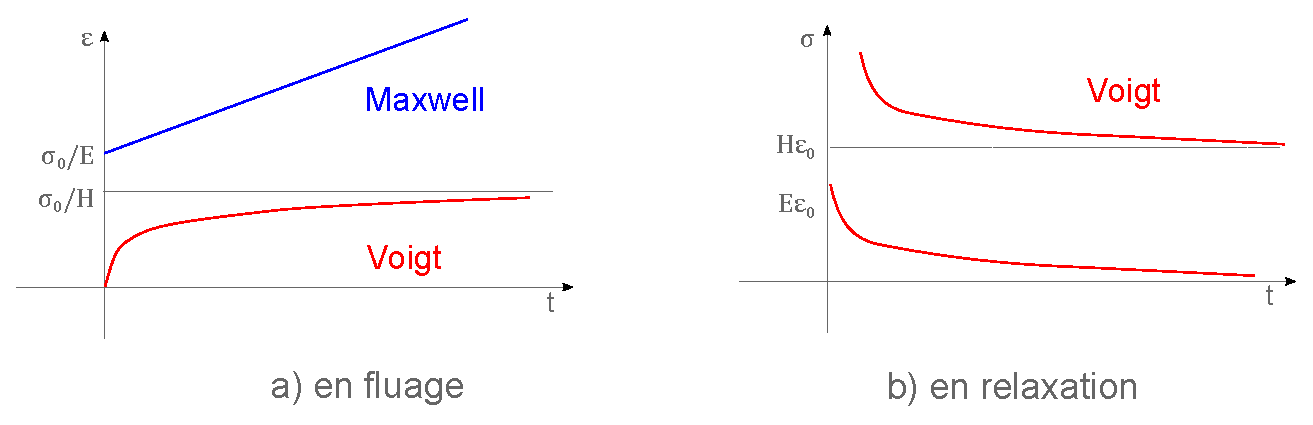
\includegraphics[height=45mm]{MaxwellVoigt.eps}}
\caption{Modèles de Maxwell et Voigt}\label{Fig-MaxwellVoigt}
\end{figure}


\medskip
Le modèle de Voigt ne présente pas d'élasticité instantanée.
L'application d'un saut de déformation en $t = 0$ produit une contrainte infinie. 
Ce modèle n'est donc pas utilisable en relaxation, sauf si la mise en charge est progressive, et sera pour 
cette raison associé à un ressort pour effectuer des calculs de structure (\textcolorblue{modèle de 
Kelvin-Voigt}).\index{Loi de comportement!Kelvin-Voigt}\index[aut]{Kelvin (William Thomson, connu sous le nom de Lord -), 1924-1907, Anglais}\index[aut]{Voigt (Woldemar), 1850-1919, Allemand}

De plus, sous l'effet d'une contrainte $\sigma_0$ constante en fonction du temps, la déformation 
dans ce modèle de Voigt tend vers la valeur asymptotique $\sigma_0/H$: le fluage est donc limité.
Si, après une mise en charge lente, la déformation est fixée à une valeur $\varepsilon_0$, 
la contrainte asymptotique sera $H\varepsilon_0$ : il n'y a donc pas disparition complète de la
contrainte.

Au contraire, dans le cas du modèle de Maxwell,\index[aut]{Maxwell (James Clerk), 1831-1879, Écossais}
\index{Loi de comportement!Maxwell} la vitesse de fluage est constante, et la disparition de 
contrainte au cours de la relaxation est totale.



\medskip
\subsection{Plasticité}\index{Loi de comportement!Plasticité}

Les modèles présentés jusqu'à présent étaient des modèles unidimensionnels, ou plus exactement
des modèles correspondant à un \textcolorblue{chargement uniaxial}.
Pourtant, l'étude de ces modèles uniaxiaux (simples) met en évidence la détermination de
seuils ou de limites correspondant à des modifications de comportement.
Afin de pouvoir aborder l'étude des chargements multiaxiaux, il est nécessaire de se donner les
moyens de \textcolorblue{définir de telles limites dans le cas tridimensionnel}. 
C'est ce que nous allons maintenant aborder.

\medskip
Considérons le cas du chargement uniaxial d'un matériau isotrope.
Celui-ci fait apparaître un domaine d'élasticité au travers de deux valeurs de contrainte, l'une en traction, 
l'autre en compression, pour lesquelles se produit l'écoulement plastique.
On a donc élasticité dans un domaine $[-\sigma_y,\sigma_y]$, puis plasticité au delà, i.e. par exemple
pour une contrainte $>\sigma_y+x$, où $x=H\varepsilon_p$.

En fait, la limite du domaine de plasticité est défini par une \textcolorblue{fonction de charge $f$}
de sorte que si $f(\sigma,x)<0$ l'état de contrainte est élastique, et si $f(\sigma,x)>0$
l'état de contrainte est plastique.

\medskip
Dans le cas général, l'ensemble des paramètres de départ $A_I$ contiendra les contraintes et toutes 
les variables d'écrouissage, scalaires ou tensorielles, il faut donc définir $f(\sigma, A_I)$. 
On va dans un premier temps limiter la présentation à la définition du domaine d'élasticité initial, 
pour lequel on supposera que les variables $A_I$ sont nulles, si bien qu'on se contentera d'écrire les 
restrictions des fonctions $f$ dans l'espace des contraintes.

L'expérience montre que, \textcolorblue{pour la plupart des matériaux, le domaine d'élasticité initial est 
convexe} (c'est en particulier vrai pour les métaux qui se déforment par glissement cristallographique). 
La fonction de charge doit donc elle-même être convexe en $\sigma$, ce qui implique, pour tout 
réel $\lambda$ compris entre 0 et 1, et pour un couple $(\sigma_1, \sigma_2)$ quelconque de la frontière:
\begin{equation} f (\lambda\sigma_1 + (1-\lambda)\sigma_2) \le \lambda f(\sigma_1) + (1-\lambda) f(\sigma_2) \end{equation}

\textcolorblue{Il faut également respecter les symétries matérielles.}
Ceci implique en particulier dans le cas d'un matériau isotrope que $f$ soit une fonction symétrique des 
seules contraintes principales, ou bien encore, ce qui est équivalent, des invariants du tenseur des contraintes
présentés au paragraphe \ref{Sec-TensS} (il s'agit de $I_1$, $I_2$ et $I_3$).

\medskip
Dans les matériaux métalliques on observe généralement l'incompressibilité plastique ($\varepsilon^p_{ii} = 0$) 
et l'indépendance du comportement vis-à-vis de la pression isostatique. Ceci amène à considérer 
comme variable critique à faire figurer dans la définition du critère non plus le tenseur de contraintes lui-même, 
mais son déviateur $s$ (et donc ses invariants $J_1$, $J_2$ et $J_3$).

En vue de réaliser les comparaisons avec les résultats expérimentaux, il est pratique de disposer d'expressions 
des critères dans lesquelles les valeurs de $f$ sont homogènes à des contraintes.
On peut alors remplacer $J_2$ par l'invariant $J$ (contrainte équivalente au sens de von Mises en cisaillement: 
$J(\sigma)=\sigma_e= \sqrt{3J_2}$), qui peut également s'exprimer en fonction des contraintes principales, 
ou de la contrainte appliquée dans le cas d'un état de traction simple.

\medskip
Nous allons maintenant présenter quelques critères classiques de plasticité: von Mises et Trasca, ne faisant 
pas intervenir la pression isostatique, Drucker-Prager, Mohr-Coulomb, Hill et Tsaï, faisant intervenir
la pression isostatique.

Introduire la pression isostatique permet d'exprimer le fait qu'une contrainte isostatique de compression 
rend plus difficile la déformation plastique, ce qui conduit à une dissymétrie des critère en 
traction/compression.

\begin{histoire}
Un critère de plasticité, ou critère d'écoulement plastique, est un critère permettant de savoir, sous des sollicitations données, 
si une pièce se déforme plastiquement ou si elle reste dans le domaine élastique. 
De nombreux essais ont montré que l'on pouvait utiliser deux critères principaux : le critère de von Mises\index[aut]{Mises (Richard Edler, von -), 1883-1953, Autrichien} 
(critère de l'énergie de distorsion élastique) ou le critère de Tresca\index[aut]{Tresca (Henri Édouard), 1814-1885, Français}  
(critère de la contrainte de cisaillement maximal).
En résistance des matériaux, on désire parfois rester dans le domaine élastique, on parle alors de critère de résistance.

La contrainte de comparaison n'est pas une contrainte réelle existant à un instant donné à l'intérieur d'un solide, mais est utilisée 
en mécanique pour prédire la rupture. Néanmoins, la plupart des ingénieurs l'utilisent pour déterminer si un champ de contrainte 
donné dans une pièce est acceptable ou non. On parle aussi de contrainte équivalente ou de contrainte effective. Elle découle des 
critères de plasticité.

Cette contrainte est comparée à la limite d'élasticité ou encore la contrainte de rupture obtenue par essai de traction.

\medskip
Le critère dit de von Mises\index[aut]{Mises (Richard Edler, von -), 1883-1953, Autrichien}\index{Critère de plasticité!von Mises} 
a été formulé initialement par Maxwell en 1865.\index[aut]{Maxwell (James Clerk), 1831-1879, Écossais} 
En 1904, Huber\index[aut]{Huber (Tytus Maksymilian), 1872-1950, Polonais} le développa partiellement dans un 
article en polonais. 
Cependant, sa paternité est généralement attribuée à von Mises (1913).\index[aut]{Mises (Richard Edler, von -), 1883-1953, Autrichien}
On parle aussi parfois de la théorie de Maxwell-Huber-Hencky-von Mises,\index[aut]{Hencky (Heinrich), 1885-1951, Allemand} 
ou de critère de Prandtl-Reuss,\index[aut]{Prandtl (Ludwig), 1875-1953, Allemand}\index[aut]{Reuss}
ou encore de critère de l'énergie de distorsion élastique.

\medskip
La renommée de Tresca\index[aut]{Tresca (Henri Édouard), 1814-1885, Français} 
était si grande à son époque que Gustave Eiffel\index[aut]{Eiffel (Gustave), 1832-1923, Français} 
mit son nom en troisième  position sur la Liste des soixante-douze noms de savants inscrits sur la tour Eiffel,
et plus précisemment sur le pilier face au Trocadéro.

\medskip
Sur ce même pilier (comportant 18 noms), en plus des mathématiciens Lagrange,\index[aut]{Lagrange (Joseph Louis, comte de -), 1736-1813, Italien} 
Laplace,\index[aut]{Laplace (Pierre Simon de -), 1749-1827, Français} Legendre\index[aut]{Legendre (Adrien-Marie), 1752-1833, Français} 
et Chasles,\index[aut]{Chasles (Michel), 1793-1880, Français} se trouve
également Navier.\index[aut]{Navier (Claude Louis Marie Henri), 1785-1836, Français} 
Celui-ci n'apparaît pas pour ses contributions aux mathématiques et à la physique\footnote{%
Lorsque, en 1822, il modifia les équations d'Euler pour décrire un fluide en incluant la viscosité, son raisonnement
mathématique était erroné, mais par chance, ou grâce à son intuition, il obtint malgré tout les bonnes
équations. Le raisonnement rigoureux fut trouvé quelques années plus tard par le mathématicien irlandais 
Stokes\index[aut]{Stokes (George Gabriel), 1819-1903, Anglais}}, mais
parce qu'il était considéré lui-aussi comme l'un des plus grands ingénieurs français et comme personnage
public important: de 1830 à sa mort en 1836, il fut employé par le gouvernement français comme consultant
afin de permettre à la France de progresser grâce aux sciences et aux technologies.
\end{histoire}


\medskip
\subsubsection{Critère de von Mises}

Dans le \textcolorblue{critère de von Mises},\index[aut]{Mises (Richard Edler, von -), 1883-1953, Autrichien} 
on considère que le seuil de plasticité est lié à l'énergie élastique de
cisaillement. Cela revient à négliger l'influence du troisième invariant. 
Si $\sigma_y$ est la limite d'élasticité en traction, la fonction de charge est définie par:
\begin{equation} f(\sigma) = J(\sigma) - \sigma_y \end{equation}

La direction d'écoulement est donnée par le déviateur du tenseur des contraintes.

\medskip
\subsubsection{Critère de Tresca}

Le \textcolorblue{critère de Tresca},\index[aut]{Tresca (Henri Édouard), 1814-1885, Français} \index{Critère de plasticité!Tresca} 
ou critère de Tresca-Guest,\index[aut]{Guest} ou critère de la contrainte de 
cisaillement maximal, s'exprime en fonction des cisaillements maxima dans chaque plan principal, représentés 
par les quantités $(\sigma_i-\sigma_j)$ (et non plus à l'énergie élastique de cisaillement).

La spécificité du critère de Tresca est de ne retenir que le plus grand d'entre eux. Le fait
de rajouter une pression à chaque terme de la diagonale ne modifie pas, comme prévu, la valeur du critère.
Contrairement au critère de von Mises, l'expression du critère de Tresca ne définit en général pas une 
surface régulière (discontinuité de la normale, points anguleux):
\begin{equation} f(\sigma) = \max(\sigma_i - \sigma_j) - \sigma_y \end{equation}
En d'autres termes, la loi d'écoulement se définit par secteurs dans l'espace des contraintes principales.


\medskip
\subsubsection{Critère de Drucker-Prager}

\textcolorgris{On trouve parfois \og Drücker\fg{} au lieu de \og Drucker\fg{} dans la
littérature.}

\medskip
La fonction de charge s'écrit $f(\sigma)=(1-\alpha)J(\sigma)+\alpha tr(\sigma)$, si
bien que la normale possède une composante shérique.
La déformation plastique évaluée avec un tel critère est accompagnée d'une
augmentation de volume quel que soit le chargement appliqué.

De manière générale, tout critère qui fait apparaître la pression isostatique
produit un terme de changement de volume accompagnant la déformation plastique (mais
pas forcément positif, comme dans le cas du modèle de Drucker-Prager\index{Critère de plasticité!Drucker-Prager}\index[aut]{Drucker (Daniel Charles), 1918-2001, Américain}\index[aut]{Prager (William), 1903-1980, Américain} 
qui comporte donc un défaut).

On l'écrit aussi sous une forme où il est plus facile de le voir comme une extension du critère de von Mises:\index[aut]{Mises (Richard Edler, von -), 1883-1953, Autrichien}\index{Critère de plasticité!von Mises}
\begin{equation} f(\sigma) = J(\sigma) - \dfrac{\sigma_y-\alpha I_1}{1-\alpha} \end{equation}
où le coefficient $\alpha$ dépend du matériau et est compris entre 0 et $1/2$. Pour
$\alpha=0$, on retrouve le critère de von Mises.

\medskip
\subsubsection{Critère de Mohr-Coulomb}

Ce critère\index{Critère de plasticité!Mohr-Coulomb}\index[aut]{Mohr (Christian Otto), 1835-1918, Allemand}\index[aut]{Coulomb (Charles-Augustin), 1736-1806, Français} 
est apparenté à celui de Tresca,\index{Critère de plasticité!Tresca}\index[aut]{Tresca (Henri Édouard), 1814-1885, Français} 
car il fait intervenir comme lui le cisaillement maximum, mais, contrairement à lui, il ajoute en même temps 
la contrainte \og moyenne\fg{}, représentée par le centre du cercle de Mohr correspondant au cisaillement 
maximum, soit:
\begin{equation} f(\sigma) = \sigma_1 - \sigma_3 + (\sigma_1 + \sigma_3) \sin\varphi - 2C\cos \varphi \quad
\text{ avec } \quad \sigma_3 \le \sigma_2 \le \sigma_1 \end{equation}
Ce critère est sous-tendu par la notion de frottement, et suppose que le cisaillement maximal que peut 
subir le matériau est d'autant plus grand que la contrainte normale de compression est élevée.

\medskip
\subsubsection{Critères anisotropes}

La méthode généralement utilisée pour faire apparaître de l'anisotropie consiste à faire intervenir 
un tenseur du quatrième ordre dans l'expression du critère, qui vient multiplier le déviateur, ou directement 
le tenseur des contraintes. 

Une solution couramment adoptée généralise le critère de von Mises, en utilisant à la place de $J(\sigma)$ 
l'expression : $J_H(\sigma) = \sqrt{\sigma : H : \sigma}$.

\medskip
Le \textcolorblue{critère de Hill}\index[aut]{Hill (Rodney), 1921-2011, Anglais}\index{Critère de plasticité!Hill} 
correspond à une anisotropie particulière qui conserve trois plans de  symétrie dans l'état d'écrouissage du 
matériau. 

\medskip
Le \textcolorblue{critère de Tsaï}\index{Critère de plasticité!Tsaï}\index[aut]{Tsaï (Stephen W), ?-, Américain} 
est obtenu à partir de celui de Hill afin de représenter la dissymétrie entre traction et compression.







\medskip
\subsection{Les élastomères}\index{Loi de comportement!Élastomères}

Dans ce paragraphe, nous faisons une présentation sommaire des élastomères de manière
générale.

\medskip
Le comportement des élastomères est fortement non linéaire.
Il faut prendre en compte par exemple la précharge, la fréquence et l'amplitude
d'excitation comme paramètres sur :
\begin{itemize}
	\item en statique : très grandes déformations et retour à la configuration
		initiale sans déformation permanente : lois hyperélastiques.
	\item en dynamique : propriétés amortissantes, dont rigidification en fréquence
		sous excitation harmonique : loi viscoélastique non linéaire.
\end{itemize}

\medskip
Concernant leur fabrication, l'opération de \textcolorblue{vulcanisation} est la suivante: 
on malaxe du caoutchouc brut, on ajoute du souffre et on chauffe le
mélange afin d'obtenir un matériau élastique, stable dans une gamme de température
beaucoup plus large que le caoutchouc naturel et résistant au fluage sous contrainte 
(découverte de Goodyear en 1839).\index[aut]{Goodyear (Charles), 1800-1860, Américain}

Le premier brevet sur la fabrication d'un élastomère synthétique a été déposé le 12 septembre 
1909 par le chimiste allemand Fritz Hofmann.\index[aut]{Hofmann (Friedrich Carl Albert dit Fritz), 1866-1956, Allemand}

\medskip
Les élastomères sont \textcolorblue{quasi incompressibles}.
le module de compressibilité du caoutchouc se situe entre 1000 et 2000 MPa alors
que l'ordre du grandeur de son module de cisaillement est de 1 MPa : cette différence
signifie que le caoutchouc ne change quasiment pas de volume, même sous de
fortes contraintes.

\medskip
\textcolorblue{Les déformations de cisaillement peuvent être considérées comme linéaires:}
le coefficient de cisaillement est relativement indépendant du taux de cisaillement, au moins
jusqu'à des niveaux de déformation modérés.

\medskip
Enfin, notons également un comportement particulier, connu sous le nom d'\textcolorblue{effet 
Mullins} (publications en 1966 et 1969):\index[aut]{Mullins (Leonard)}
si l'on applique un chargement cyclique sur un matériau initialement non précontraint,
on observe une diminution de la raideur lors des premiers cycles. Si on impose ensuite une
déformation cyclique jusqu'à un niveau de déformation plus élevé, on observe
à nouveau une diminution de la contrainte et de l'hystérésis jusqu'à un
nouvel équilibre. Ce comportement provient d'une rupture progressive des
liaisons moléculaires.


\medskip
Les élastomères sont connus pour leur \textcolorblue{grande élasticité}.
Une \textcolorblue{hystérésis est toujours présente}, mais augmente avec l'ajout de charges
(qui sont nécessaires pour améliorer d'autres propriétés).

Rappelons ce qu'est l'hystérésis en quelques mots: 
l'amortissement correspond à l'énergie dissipée au cours d'un cycle. Il est 
caractérisé par un angle de perte et un module complexe.
Si le système est soumis à des déformations sinusoïdales cycliques :
$\varepsilon(t)=\varepsilon_0\sin(\omega t)$ et que l'on estime que la
contrainte transmise répond également de façon sinusoïdale, alors cette
dernière est déphasée d'un angle $\delta$, l'angle de perte, et on a :
$\sigma(t)=\sigma_0\sin(\omega t+\delta)$.
Généralement cette hypothèse de première harmonique n'est pas
vérifiée et la réponse contient plusieurs harmoniques :
$\sigma(t) = \sum_k \sigma_k\sin(k\omega t+\delta_k)$.

Le module complexe est défini par : $E^* = \sigma / \varepsilon$. Il se calcule comme :
\begin{equation} E^*=\dfrac{\sigma_0}{\varepsilon_0}e^{i\delta}=\dfrac{\sigma_0}{\varepsilon_0}(\cos\delta+i\sin\delta)\end{equation}
ou encore :
\begin{equation}
E^* = E' + i E'' = E'(1+i\tan\delta)
\end{equation}
et on appelle :
\begin{itemize}
	\item module dynamique = $|E^*|=\dfrac{\sigma_0}{\varepsilon_0}$;
	\item module de stockage = $E'=|E^*|\cos\delta$, car il mesure l'énergie
		emmagasinée puis restituée au cours d'un cycle;
	\item module de perte = $E''=|E^*|\sin\delta$, car il mesure l'énergie
		dissipée sous forme de chaleur au cours d'un cycle.
\end{itemize}
Le \textcolorblue{module d'Young complexe $E^*$ ou le module de Coulomb complexe $G^*$}
\index[aut]{Young (Thomas), 1773-1829, Anglais}\index{Module d'Young}\index[aut]{Coulomb (Charles-Augustin), 1736-1806, Français}\index{Module de Coulomb}
évoluent de manière significative avec la température, la fréquence et l'amplitude
de l'excitation.

\medskip
Notons également que l'\textcolorblue{effet mémoire} (expériences de fluage et relaxation) est présent
pour ces matériaux:
Le niveau des contraintes à un instant dépend non seulement du niveau de sollicitation
à cet instant, mais également des sollicitations auxquel le matériau a été soumis
précédemment.




\medskip
\subsubsection{Grandes déformations}
En grandes déformations, il est nécessaire de bien distinguer l'état initial de
l'état déformé.

On utilisera alors les tenseurs adaptés (Piola-Kirchhoff), comme exposé au paragraphe \ref{Sec-NLg}.

%Les variations de volume entre les configurations sont caractérisées par $J=det(F)$.

\medskip
\subsubsection{Incompressibilité}

Aux lois de comportement précédentes, on ajoute la contrainte de variation
nulle de volume entre les configurations.

Pour un matériau incompressible, on  a $J=1$ ($J$ est le jacobien du gradient de la déformation).




\medskip
\subsubsection{Hyperélasticité}\index{Loi de comportement!Hyperélasticité}

Un matériau est dit élastique si le tenseur des contraintes de Cauchy à l'instant $t$
dépend uniquement de l'état de déformation à ce même instant : la contrainte ne
dépend pas du chemin suivi par la déformation, alors que le travail fourni par cette
contrainte en dépend.

Un matériau élastique est dit \textcolorblue{hyperélastique} si le tenseur des contraintes dérive
d'une \textcolorblue{fonction d'énergie} de ce matériau: cela implique que le travail fourni pour aller 
d'un état à un autre ne dépend pas du chemin suivi.

Si on postule l'existence d'une \textcolorblue{énergie libre $\Psi$}, on peut la relier, pour les matériaux
hyperélastiques, aux invariants des tenseurs. Cette énergie est également appelée énergie de 
déformation. De là on peut déduire les lois de comportement.




\medskip
\subsubsection{Approximation numérique}

De nombreuses formes de l'énergie de déformation ont été proposées, s'exprimant à partir :
\begin{itemize}
	\item des invariants;
	\item des fonctions d'élongations principales;
	\item des coefficients intervenant sous forme linéaire : Mooney-Rivlin\index[aut]{Mooney (Melvin), 1893-1968, Américain} 
	et Rivlin généralisé;\index[aut]{Rivlin (Ronald Samuel), 1915-2005, Américain}
	\item des coefficients intervenant sous forme de puissances : Ogden (1972)\index[aut]{Ogden (Ray W.)}
	\item sous forme polynomiale...
\end{itemize}

\medskip
Le \textcolorblue{modèle de Rivlin généralisé},\index[aut]{Rivlin (Ronald Samuel), 1915-2005, Américain}\index{Loi de comportement!Rivlin généralisé} 
implémenté dans la plupart des codes de calcul, est donné par le développement polynomial suivant :
\begin{equation}
\Psi = \dsum\limits_{i,j=0}^N C_{ij}(I_1-3)^i(I_2-3)^j + \dsum_{i=1}^M D_i(J-1)^{2i}
\end{equation}
ou plus simplement, si le matériau est bien incompressible:
\begin{equation}
\Psi = \dsum\limits_{i,j=0}^N C_{ij}(I_1-3)^i(I_2-3)^j
\end{equation}
où l'énergie de déformation est développée à un ordre proportionnel à la plage
de déformation souhaitée (pour $N=3$ on a généralement une bonne corrélation
avec les mesures expérimentales).
$C_{00}=0$ et les coefficients $C_{ij}$ sont des constantes du matériau liées à sa réponse
en terme de distortion, et les coefficients $D_i$ sont des constantes du matériau liées à sa réponse
en terme de volume.

\medskip
Pour les matériaux faiblement compressibles, il est commode d'introduire la
décomposition des déformations.
On en arrive alors à la forme :
\begin{equation}
\Psi(J) = \dsum\limits_{i=1}^N \dfrac1{D_i}(J-1)^{2i}
\end{equation}
le module de compressibilité étant donné par $k_0=2/D_1$.


\medskip
Notons qu'une manière également simple de prendre en compte les élastomère a
déjà été donnée: il s'agit de l'utilisation d'éléments hybrides faisant intervenir 
la matrice de souplesse $[S]$ au lieu de la matrice de Hooke $[H]$.






\medskip
\subsection{Les composites, l'anisotropie}

Dans ce paragraphe, nous faisons une présentation sommaire des matériaux composites
de manière générale.

Ceux-ci ont fait des apparitions en divers endroits de ce document, et quelques problèmes
se rapportant à eux ont été discutés.

\medskip
\subsubsection{Définitions}

\begin{definition}[Matériau composite]
On appelle \textcolorblue{matériau composite} l'association d'au moins deux matériaux non miscibles. 
On obtient un matériau hétérogène.
\end{definition}

On en profite donc pour rappeler qu'un matériau peut être:
\begin{itemize}
	\item \emph{Homogène:} même propriétés en tout point du matériau.
	\item \emph{Hétérogène:} en 2 points différents, propriétés différentes.
	\item \emph{Isotrope:} même propriétés dans toutes les directions.
	\item \emph{Isotrope transverse:} il existe un axe de symétrie. Symétrie par rapport à une droite.
	\item \emph{Orthotrope:} propriétés symétriques par rapport à deux plans orthogonaux.
	\item \emph{Anisotrope:} les propriétés sont différentes selon les différentes directions. 
\end{itemize}

\medskip
\subsubsection{Composants}

Un matériau composite plastique correspond à l'association de deux constituants .
\begin{itemize}
	\item Le \textcolorblue{renfort} (ou armature, ou squelette): assure la tenue mécanique (résistance à la 
		traction et rigidité). Souvent de nature filamentaire (des fibres organiques ou inorganiques).
	\item La \textcolorblue{matrice}: lie les fibres renforts, répartit les efforts (résistance à la compression 
		ou à la flexion), assure la protection chimique. Par définition, c'est un polymère ou 
		une résine organique.
\end{itemize}

\medskip
En plus de ces deux constituants de base, il faut ajouter l'\textcolorblue{interphase}, qui est l'interface 
assurant la compatibilité renfort-matrice, et qui transmet les contraintes de l'un à l'autre sans
 déplacement relatif.

\medskip
Des produits chimiques entrent aussi dans la composition du composite, l'interphase etc. ... 
qui peuvent jouer sur le comportement mécanique, mais n'interviennent pratiquement
jamais dans le calcul de structure composite.

\medskip
\colorgreen Remarque : on conçoit un composite en fonction du type d'application, de chargement... ce qui est différent
des matériaux classiques où on adapte la conception d'une structure en fonction du matériau constitutif.
On cherchera donc toujours à orienter au mieux les renforts en fonction des efforts auxquels la structure 
est soumise.\colorblack

\medskip
\textcolorblue{Avantages} des matériaux composites :
\begin{itemize}
	\item  grande résistance à la fatigue;
	\item  faible vieillissement sous l'action de l'humidité, de la chaleur, de la corrosion (sauf alu-carbone);
	\item  insensibles aux produits chimiques \og mécaniques\fg{} comme les graisses, huiles, liquides hydrauliques,
		 peintures, solvants, pétrole;
\end{itemize}
Mais attention aux décapants de peinture qui attaquent les résines époxydes !


\medskip
\subsubsection{Les matériaux composites structuraux}

\begin{itemize}
	\item  Les \textcolorblue{monocouches} représentent l'élément de base de la structure composite.
		 Les différents types de monocouches sont caractérisés par la forme du renfort :
		 à fibres longues (unidirectionnelles UD, réparties aléatoirement), à fibres tissées,
		 à fibres courtes.
	\item  Un \textcolorblue{stratifié} est constitué d'un empilement de monocouches ayant chacun une orientation
		 propre par rapport à un référentiel commun aux couches et désigné comme le
		 référentiel du stratifié.
	\item Un matériau \textcolorblue{sandwich} est un matériau composé de deux \textcolorblue{peaux}
		 de grande rigidité et de faible épaisseur enveloppant une \textcolorblue{âme (ou cœur)} 
		de forte épaisseur et faible résistance. 
		L'ensemble forme une structure d'une grande légèreté. 
		Le matériau sandwich possède une grande rigidité en flexion et est un excellent isolant
		 thermique.
\end{itemize}

\medskip
On pourra avoir des stratifiés de \textcolorblue{type}:
\begin{itemize}
	\item  \emph{Equilibré}: stratifié comportant autant de couches orientée suivant la direction
		$+\theta$ que de couches orientée suivant la direction $-\theta$.
	\item \emph{Symétrique}: stratifié comportant des couches disposées symétriquement par
		 rapport à un plan moyen.
	\item \emph{Orthogonal}: stratifié comportant autant de couches à $0^o$ que de couches à $90^o$.
	\item Notation \og composite \fg{} :
		On porte, entre crochets, un nombre indiquant la valeur en degré de l'angle que fait la direction 
		des fibres de chaque couche avec l'axe de référence. les couches sont nommées successivement 
		en allant de la face inférieure à la face supérieure, les couches étant séparées par le symbole 
		\og /\fg{} (ou une virgule parfois): $[0/+45/+90/-45]$

		Les couches successives d'un même matériau et de même orientation sont désignées
		par un indice: $[0/45/45/90/-45/-45/0]$ s'écrit $[0/45_2/90/-45_2/0]$.
		
		Si le stratifié est symétrique, seule la moitié est codifiée et le symbole \og s\fg{} indique 
		la symétrie: $[-45/45/-45/-45/45/-45]$ s'écrit $[-45/45/-45]_s$.

		En cas de stratification hybride (différents matériaux dans un même stratifié), il faut
		préciser par un indice la nature de la couche.
\end{itemize}


\medskip
\subsubsection{Approximation numérique}\index{Loi de comportement!Anisotrope}

L'ingénieur mécanicien est souvent bien au fait des diverses approximations possibles d'un 
matériau composite. Nous serons par conséquent assez brefs sur le sujet.

Par ailleurs le chapitre \ref{Ch-Homog} sur l'homogénéisation permet, dans certains cas, de remplacer
un matériau composite compliqué par un matériau homogénéisé plus simple.

\medskip
La loi de Hooke, telle qu'elle a été écrite jusqu'\ a présent $\sigma=H\varepsilon$ ne s'oppose
aucunement à l'anisotropie. 

L'isotropie se traduit juste par le fait que plus de coefficients sont nuls, 
et que ceux qui sont non nuls ne dépendent que de deux paramètres, comme rappelé 
en introduction au paragraphe \ref{Sec-NLMat}.

\medskip
Lorsque le matériau est \textcolorblue{anisotrope}, alors $H$ peut être pleine, ce qui correspond à
\textcolorblue{21 coefficients} non nuls, dépendant des paramètres :
$E_i$ : modules de tensions, $G_{ij}$ : modules de cisaillement, $\nu_{ij}$ : coefficients de contraction,
$\eta_{ij,k}$ : coefficients d'influence de 1ère espèce, $\eta_{i,kl}$ : coefficients d'influence de 
2nde espèce, et $\nu_{ij,kl}$: coefficients de Chentsov.

L'\textcolorblue{orthotropie} (orthogonal et anisotrope, i.e. 2 plans orthogonaux de symétrie) fait descendre 
ce nombre de coefficients non nuls à \textcolorblue{9}, dépendant des paramètres: $E_1, E_2, E_3$: 
modules d'élasticité longitudinaux, $G_{23}, G_{13}, G_{12}$: modules de cisaillement, $\nu_{23}, \nu_{13},
 \nu_{12}, \nu_{21}, \nu_{23}, \nu_{31}$: coefficients de Poisson.

L'\textcolorblue{isotropie transverse} (1 axe de symétrie) fait encore descendre ce nombre de 
coefficients non nuls à \textcolorblue{6} (on n'a plus besoin de $E_2$, $G_{23}$ et $G_{12}$ par 
exemple)

\medskip
On peut également faire des hypothèses sur l'épaisseur des plis (faible) et la répartition des contraintes
ou déformations pour obtenir des théories de plaques équivalentes.
Ces plaques équivalentes pouvant ensuite être assemblées en une nouvelle plaque équivalente.

\medskip
Chaque coefficient non nul peut lui-même être constant (élasticité anisotrope) ou non, permettant
de prendre en compte autant de comportements que nécessaire (viscoélasticité, plasticité...).
En sus, il est également nécessaire de \textcolorblue{judicieusement modéliser l'interphase}, i.e. de bien
décrire comment les couches peuvent ou non bouger entre elles. Par défaut, l'hypothèse
utilisée dans les codes de calcul est une adhésion parfaite. Cela n'est pas forcément compatible
avec le but recherché par le calcul, notamment si celui-ci vise à appréhender les modes
de rupture (qui sont plus complexes pour les composites...).

\medskip
Tous les codes de calcul actuels permettent de prendre en compte l'anisotropie matérielle
et les matériaux composites (avec des interfaces plus ou moins sympathiques).
Nous n'entrerons donc pas plus dans le détail dans ce document.






\medskip
\section{Le contact}\label{Sec-contact}

\medskip
\begin{histoire}%
Les premiers calculs de Joseph Boussinesq,\index[aut]{Boussinesq (Joseph Valentin), 1842-1929, Français} 
auteur en 1876 d'un \emph{Essai théorique de l'équilibre des massifs pulvérulents, comparé à celui des 
massifs solides, sur la poussée des terres sans cohésion}, reprenant des études de 
Coulomb\index[aut]{Coulomb (Charles-Augustin), 1736-1806, Français} sur ce sujet, reposent sur 
un ensemble d'hypothèses très restrictives: 
%\begin{enumerate}
%   \item 
1) les corps en présence sont supposés semi-infinis (cela n'est vrai que si les zones de contact sont 
vraiment très petites par rapport aux autres dimensions);
%   \item 
2) au voisinage de la future zone de contact, leurs surfaces peuvent être représentées par des 
quadriques dont les courbures sont connues (Or la rugosité, qui rend la répartition des pressions 
de contact très irrégulière, est généralement très éloignée du modèle théorique);
%   \item 
3) ces corps sont parfaitement élastiques, homogènes et isotropes (ce qui est très restrictif,
et souvent réellement faux);
%   \item 
4) l'aire de contact est assimilée à un très petit élément plan qui ne reçoit que des efforts 
normaux, donc parallèles entre eux (dans beaucoup de contacts, la zone d'application des pressions 
est loin d'être plane et surtout, le fait de ne considérer que des charges normales suppose que l'on 
fasse abstraction du frottement).
%\end{enumerate}

\medskip
En 1881, Heinrich Hertz,\index[aut]{Hertz (Heinrich Rudolf), 1857-1894, Allemand} jeune ingénieur et 
docteur ès sciences de 24 ans, publie dans le célèbre Journal de Crelle (XVII, p. 156) sous le titre 
\emph{\"Uber die Beruhrung fester elastischer Körper}  (Sur le contact des corps solides élastiques), 
un mémoire qui fera date, puisqu'il s'agit de la première théorie cohérente des contacts ponctuels.

\sbox{\MaBoiteAvecPhotos}{\setlength{\tabcolsep}{0pt}\scriptsize%
\begin{tabular}{ccc}%
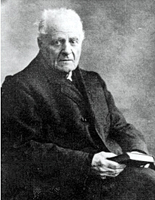
\includegraphics[height=\the\HauteurDesPhotos]{Boussinesq}&%
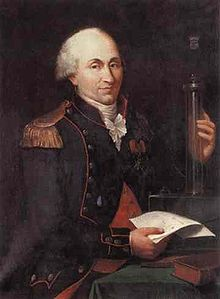
\includegraphics[height=\the\HauteurDesPhotos]{Coulomb}&%
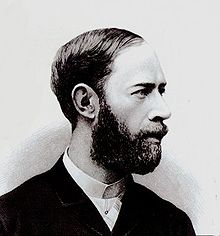
\includegraphics[height=\the\HauteurDesPhotos]{Hertz}\\
Boussinesq&%Coulomb&%Hertz%
\end{tabular}}
\medskip
\ImageADroite{%
Le fait de rester dans le domaine des déformations élastiques permet d'appliquer le principe de 
superposition: 
aux contraintes issues de 1) l'application des efforts normaux se superposent celles 2) provoquées 
par les efforts tangentiels résultant du frottement ou de l'adhérence, puis celles 3) dues aux contraintes 
résiduelles dont on favorise l'apparition par des traitements mécaniques ou thermochimiques appropriés, 
et enfin celles 4) qui correspondent aux autres sollicitations des pièces, tension, compression, flexion, torsion...
Ces quatre groupes de contraintes peuvent être définis séparément puis combinés pour aboutir 
à l'état de charge complet des zones de contact.
}

\medskip
Le calcul des contraintes supplémentaires dues au frottement a été conduit de diverses manières 
par des chercheurs comme Liu (1950), 
Poritzky\index[aut]{Poritsky (H.),} (1966) et quelques autres. 
Il est extrêmement compliqué, au point d'être pratiquement inutilisable dans les situations 
concrètes. 
\end{histoire}
\colorblack

\medskip
Depuis que Hertz\index[aut]{Hertz (Heinrich Rudolf), 1857-1894, Allemand} a introduit une théorie 
du contact en 1881, de nombreux problèmes  d'ingénieur faisant intervenir le contact ont été résolus. 
L'outil de calcul basé sur une approche analytique, est limité à la résolution des problèmes 
simples de contact: en effet la plupart des solutions analytiques supposent un contact sans frottement 
et des zones de contact connues, à priori, et des formes géométriques simples. 

Le développement des techniques numériques de résolution a permis de traiter des
problèmes de contact plus complexes. 
La MEF, en permettant la discrétisation des solides de formes quelconques et la prise en 
compte aisée de conditions aux limites diverses, offre un outil puissant de calcul pour 
étudier les problèmes de contact.

\medskip
Aujourd'hui l'analyse des problèmes de contact avec frottement est très importante 
pour beaucoup d'applications industrielles. 
La modélisation des procédés industriels de mise en forme, et plus généralement des 
phénomènes complexes où le contact et le frottement s'ajoutent à des non-linéarités 
du matériau et de la géométrie, nécessite des algorithmes supplémentaires dans les 
logiciels généraux d'EF.

\medskip
\textcolorred{Malgré la linéarité de la loi élastique, le problème de contact est 
intrinsèquement non-linéaire. 
En effet, la surface de contact et les forces de contact sont, à priori, inconnues et elles changent 
progressivement lorsqu'on applique le chargement externe.}

\medskip
Dans la littérature, de nombreuses méthodes ont été développées pour résoudre les problèmes 
de contact par des méthodes numériques comme la MEF, parmi lesquels la méthode de pénalisation, 
la méthode de flexibilité, la méthode de programmation mathématique, la méthode des 
multiplicateurs\index{Multiplicateurs de Lagrange} de 
Lagrange\index[aut]{Lagrange (Joseph Louis, comte de -), 1736-1813, Italien} 
(voir le paragraphe \ref{Sec-MultLag} sur les multiplicateurs de Lagrange et le
paragraphe \ref{Sec-interf} sur les diverses manières de traiter une interface, qui est un
contact rigide).
Une grande partie de ces articles traitent d'algorithmes numériques. 
Dans les codes EF industriels (Ansys, Pamcrash...), les problèmes de contact avec frottement dans le 
contexte des grandes déformations sont presque exclusivement traités par des méthodes de pénalisation 
ou de régularisation. Ces méthodes présentent des inconvénients en ce qui concerne la stabilité 
et la précision numérique, en particulier pour tout ce qui touche à la simulation des phénomènes de 
frottement.

\medskip
Pour pallier ces insuffisances, une méthode du Lagrangien Augmenté a été développée par 
Curnier\index[aut]{Curnier (Alain), 1948-, Suisse} et Alart\index[aut]{Alart (Pierre), ?-, Français} (1988).
Cette méthode consiste à déterminer les inconnues (déplacement et réaction) simultanément en 
utilisant un algorithme de Newton généralisé. 
Simo\index[aut]{Simo (Juan-Carlos), 1952-1994, Espagnol} et 
Laursen\index[aut]{Laursen (Tod A), ?-, Américain} ont également proposé une méthode similaire (1992). 
De Saxcé\index[aut]{De Saxé (Géry), 1955-, Français} et 
Feng\index[aut]{Feng (Zhi-Qiang), 1963-, Français} ont proposé une méthode bipotentielle fondée 
sur la théorie du Matériau Standard Implicite, dans laquelle une nouvelle formulation du lagrangien 
augmenté est développée. 

Pour les problèmes de contact unilatéral avec frottement, la méthode bipotentielle n'utilise qu'un seul 
principe variationnel sur le déplacement et une seule inégalité. 
Ainsi, le contact unilatéral et le frottement sont couplés. 
Cette nouvelle approche étend également la notion de loi normale aux comportements dissipatifs non 
associés, en tenant compte du frottement. 
Cette approche variationnelle est plus simple que l'approche classique qui inclue deux principes variationnels 
et deux inégalités respectivement pour le contact unilatéral et le frottement. 
Dans la méthode bipotentielle, le problème de contact avec frottement est traité dans un système 
réduit par un algorithme d'Uzawa à une seule phase de prédiction-correction sur le cône de frottement. 
L'extension de cette méthode dans le contexte de grandes déformations a été réalisé.
Pour être capable de traiter des problèmes industriels qui font intervenir le contact, il est important 
de disposer d'un éventail d'algorithmes afin de pouvoir moduler l'utilisation de chaque méthode selon leurs 
avantages et inconvénients dans chaque cas concret. 

\medskip
\subsection{Lois de contact et de frottement}

Considérons deux solides déformables $\Omega_1$ et $\Omega_2$ en contact en certains
points de leurs frontières. 
Soient $v$ la vitesse relative locale en un point $P$ de $\Omega_1$ par rapport à $\Omega_2$, 
et $r$ la réaction que subit $\Omega_1$ de la part de $\Omega_2$. 
Supposons défini $n$ le vecteur unitaire normal dirigé vers $\Omega_1$. 
La projection orthogonale du point $P$ sur la surface de $\Omega_2$ définit un point $P'$, dit 
\og point projeté de P\fg{}, qui sera l'origine du repère local du contact $(t_1, t_2, n)$,
comme illustré à la \fig{Fig-rep-contact}.
\begin{figure}[htb]
\centerline{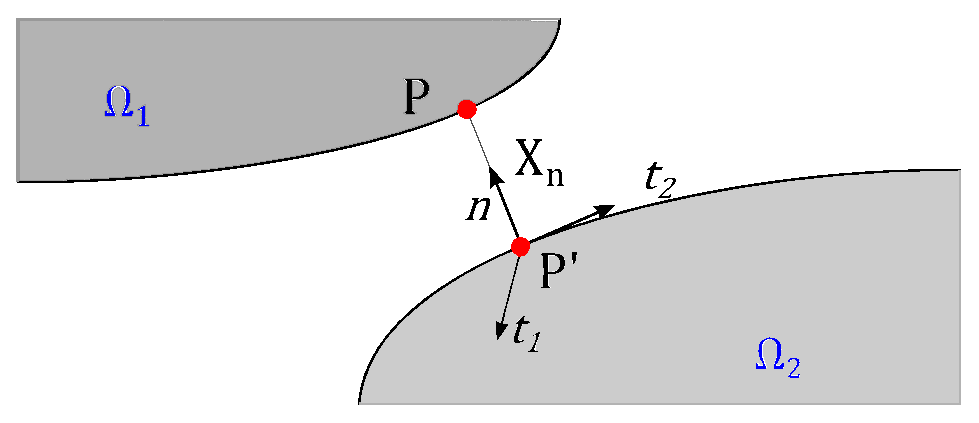
\includegraphics[height=40mm]{rep-contact.eps}}
\caption{Contact entre deux solides déformables: notations}\label{Fig-rep-contact}
\end{figure}

Les vecteurs $v$ et $r$ peuvent être décomposé en partie tangente $v_t$ et $r_t$ et partie 
normale $v_n$ et $r_n$. 

Compte tenu de la distance initiale au contact $g$ et pour un pas de temps $\Delta t$, la distance 
$PP'$ exprimée dans le repère local est alors définie par : $x_n = g + \Delta t v_n$. 
Par conséquent, les \textcolorblue{conditions de contact unilatéral} pour chaque point en contact,
peuvent être exprimées comme suit:
\begin{itemize}
   \item Impénétrabilité: $x_n \ge 0$
   \item Quand la particule est en contact avec l'obstacle, elle n'est pas attirée par lui:
	$x_n = 0 \rightarrow r_n \ge 0$
   \item Quand la particule n'est pas en contact avec l'obstacle, la réaction normale est nulle:
	$x_n > 0 \rightarrow r_n = 0$
\end{itemize}
Ces trois conditions peuvent être condensées sous une forme complémentaire (\textcolorblue{conditions 
de Signorini}):\index[aut]{Signorini (Antonio), 1888-1963, Italien}
\begin{equation} x_n \ge 0; \qquad r_n \ge 0; \qquad x_n r_n = 0 \end{equation}
ou sous la forme équivalente:
\begin{equation} \forall \rho_n > 0, \qquad r_n = proj_{R+} (r_n - \rho_n x_n) \end{equation}
où $R+$ représente un ensemble de valeurs positives.

\medskip
En ce qui concerne le frottement, parmi les nombreux modèles existants, nous avons choisi le 
\textcolorblue{modèle de Coulomb},\index[aut]{Coulomb (Charles-Augustin), 1736-1806, Français} 
qui est le plus utilisé dans les problèmes de contact avec frottement sec. 
Dans le cas du contact-frottement isotrope, le modèle de Coulomb s'écrit:
\begin{equation} \left\{\begin{array}{ll}
\|r_t\| < \mu r_n & \text{ si } \|v_t\|=0\\
r_t=-\mu r_n \frac{v_t}{\|v_t\|} & \text{ si } \|v_t\|\ne0
\end{array}\right. \end{equation}
avec $\mu$ le coefficient de frottement.

On peut également utiliser la forme équivalente:
\begin{equation}  \forall \rho_t>0, \quad r_t=proj_C (r_t-\rho_t u_t) \end{equation}
où $C$ est un ensemble qui représente l'intervalle $[-\mu r_n, \mu r_n]$ dans le cas bidimensionnel, 
ou le disque de centre $0$ et de rayon $R= \mu r_n$ dans le cas tridimensionnel.
On rapple que $u_t$ désigne la composante tangentielle du déplacement relatif, qui est
aussi le glissement.

\medskip
\subsection{Algorithme local}

De manière usuelle, on définit le \textcolorblue{cône de frottement isotrope de 
Coulomb}\index[aut]{Coulomb (Charles-Augustin), 1736-1806, Français} pour chaque point 
en contact:
\begin{equation} K_\mu = \left\{ (r_n, r_t) \in \RR^3 \text{ tels que } \|r_t\| \le \mu r_n \right\} \end{equation}

À l'aide de la théorie du Matériau Standard Implicite, les conditions de contact unilatéral et la 
loi de frottement s'expriment par une seule inégalité variationnelle:
\begin{equation} \text{Trouver } (r_n, r_t) \in K_\mu \text{ tq: }
\forall (r_n^*, r_t^*) \in K_\mu, (x_n - \mu \|v_t\|) (r_n^* - r_n) + v_t.(r_t^* - r_t) \le 0
%\end{equation}
\text{ où } \exists\lambda>0, - v_t = \lambda \frac{r_t}{\|r_t\|} \end{equation}

\medskip
Afin d'éviter des potentiels non différentiables qui apparaissent dans la représentation du contact, 
on peut utiliser la méthode du lagrangien augmenté. 
Cette méthode, appliquée à l'inégalité variationnelle, conduit à une équation implicite:
\begin{equation} r = proj_{K\mu} (r_n + \rho_n(x_n - \mu \|v_t\|), \quad r_t + \rho_t v_t) \end{equation}
où $\rho_n$ et $\rho_t$ sont des coefficients positifs qui dépendent de la matrice de flexibilité 
de contact.

Pour résoudre l'équation implicite, on utilise l'algorithme d'Uzawa\index[aut]{Uzawa (Hirofumi), 1928-, Japonais} 
(algorithme de gradient à pas fixe pour l'optimisation sous contraintes) qui conduit à une procédure 
itérative comportant les deux étapes suivantes:
\begin{itemize}
   \item prédiction: $\left\{\begin{array}{lrl} 
	\tau_n^{i+1}&=&\tau_n^i+\rho_n^i(x_n^i-\mu\|v_t^i\|)\\
	\tau_t^{i+1}&=&\tau_t^i=\rho_t^iv_t^i
	\end{array}\right.$
   \item correction: $(r_n^{i+1},r_t^{i+1}) = proj_{K\mu}(\tau_ n^{i+1}, \tau_t^{i+1})$
\end{itemize}
contact avec adhérence ($\tau\in K_\mu$), non contact ($\tau\in K_\mu^*$) et contact avec 
glissement ($\tau\in\RR^3- (K_\mu \cup K_\mu^*)$), où $K_\mu^*$ est le cône dual de $K_\mu$.

\medskip
\subsection{Algorithme global}

Dans le contexte de la MEF, après discrétisation des solides en contact, on résout généralement 
un système d'équations d'équilibre au niveau global, obtenu par la \textcolorblue{méthode des 
résidus pondérés} (exposée au paragraphe \ref{Sec-ResPond}), de type:
\begin{equation} 
\VV{R^*} = -\VV{F_{int}} + \VV{F_{ext}} + \VV{F_{reac}} = \VV{\mO} 
\end{equation}
où les vecteurs $\VV{R^*}$ des résidus, $\VV{F_{int}}$ des forces internes, $\VV{F_{ext}}$ des forces extérieures
et $\VV{F_{reac}}$ des forces de contact et de frottement dans le repère global dépendent tous du vecteur
des inconnues nodales de la structure $\VV{q}$.

\medskip
Pour résoudre ce système d'équations non linéaires, on utilise une méthode itérative
de type Newton-Raphson\index[aut]{Newton (Isaac, Sir -), 1643-1727, Anglais}\index[aut]{Raphson (Joseph), 1648-1715, Anglais}\index{Méthode de Newton-Raphson} 
qui consiste à linéariser le système précédent en:
\begin{equation} \MM{K_T}^i \VV{d}^{i+1} = -\VV{F_{int}}^i + \VV{F_{ext}}^i+\VV{F_{reac}}^i\end{equation}
\begin{equation} \VV{q}^{i+1} = \VV{q}^i+\VV{d}^{i+1} \end{equation}
où $\MM{K_T}^i$ est la \textcolorblue{matrice tangente de rigidité} à l'itération $i$.

\medskip
\textcolorred{Insistons que le caractère fortement non-linéaire de ce système}: 
en effet, celui-ci prend en compte 
des multiples non-linéarités mécaniques telles que les non-linéarités matérielles et les non-linéarités
géométriques qui se manifestent lorsqu'apparaissent des grands déplacements ou des grandes déformations. 
De plus, les lois relatives au contact et au frottement sont exprimées par des inégalités, le potentiel 
du contact étant même non différentiable. 
\textcolorred{Par conséquent, des difficultés numériques se manifestent à plusieurs niveaux au cour de:}
\begin{itemize}
   \item la résolution des équation non linéaires d'équilibre (niveau global);
   \item l'intégration des lois de comportement (niveau local);
   \item la résolution des inéquations de contact et de frottement couplées avec les équations 
	d'équilibre (niveaux local et global).
\end{itemize}


\ifVersionAvecExemplesSepares\else
   \section{Exemple: une toute première approche du contact avec \castem}

Dans ce chapitre, nous présentons un petit exemple simple de contact unidirectionnel sans frottement sous \castem.

\medskip
\subsection{Contact sur une surface infiniment rigide}

Dans ce premier exemple, nous proposons d'étudier un carré soumis sur sa face supérieure à un déplacement imposé et reposant, sur sa face inférieure, sur une surface infiniment rigide, comme illustré à la \fig{Fig-Cont0}.
\begin{figure}[ht]
  \center
  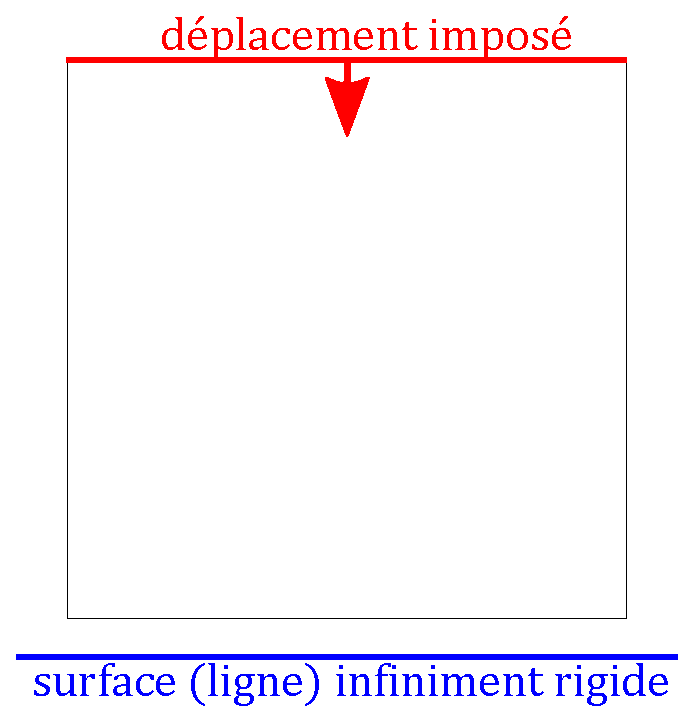
\includegraphics[height=40mm]{Contact0.eps}
  \caption{\label{Fig-Cont0} Problème de contact}
\end{figure}

\color{gris}\scriptsize
\begin{multicols}{2}
\begin{Verbatim}[numbers=left,numbersep=3pt]
OPTION ECHO 0 ;
OPTION DIME 2 ELEM QUA4 MODE PLAN CONT;
*
* Donnees
long1=10.;
nlong1=7;
uy0=-0.5;
haut1=long1;
nhaut1=nlong1;
jeu1=0.0;
*
* droite sur laquelle le carre viendra buter:
k1 = (-1.*long1) 0.;
k2 = long1 0.;
l1 = DROI (nlong1-2) k2 k1;
*
* carre:
k3 = (-0.5*long1) jeu1;
k4 = (0.5*long1) jeu1;
l2 = DROI nlong1 k3 k4;
s1 = l2 TRAN nhaut1 (0. haut1);
\end{Verbatim}
\end{multicols}
\color{black}\normalsize

\medskip
On remarquera les choses suivantes:
\begin{itemize}
  \item la ligne~$l_2$ correspondant à la face inférieure du carré «repose», sans jeu, sur la ligne~$l_1$ définissant la surface rigide sur laquelle le carré va venir buter (on aurait pu mettre un jeu initial non nul, mais ce n'est pas nécessaire);
  \item les orientations des lignes~$l_1$ et~$l_2$ sont inversées car les deux lignes en contact doivent se  «tourner le dos» au sens des normales. Cela est obligatoire;
  \item La surface de contact~$l_1$ est modélisée en utilisant~$nlong_1-2$ éléments pour le maillage, alors que le carré (ligne~$l_2$) n'en a que~$nlong_1$, afin que les maillages ne soient pas «compatibles» (i.e. que les nœuds ne tombent pas en face les uns des autres).
\end{itemize}

\color{gris}\scriptsize
\begin{multicols}{2}
\begin{Verbatim}[numbers=left,numbersep=3pt,firstnumber=last]
* Modele:
ModM1 = MODEL s1 MECANIQUE ELASTIQUE;
MatM1 = MATER ModM1 'YOUN' 1.E3 'NU' 0.3 ;
*
* CL en deplacements (Rigidites):
* 1) il faut une condition selon UX: 
*        on prend le point (0,0)
k5 = s1 POIN PROC (0. jeu1);
CLk5 = BLOQ k5 UX;
* 2) ligne de contact: rigidites
Depl1 Rigid1 = IMPO l2 l1;
Rigid2 = BLOQ DEPL l1;
* 2) ligne sur laquelle on va imposer le deplacement
l3 = s1 'COTE' 3;
CLl3 = BLOQ l3 UY ;
DCLl3 = DEPI CLl3 UY0;
* Totalite des conditions aux limites
CL0 = CLk5 ET CLl3 ET Rigid1 ET Rigid2;
\end{Verbatim}
\end{multicols}
\color{black}\normalsize

\medskip
Nous sommes en élasticité linéaire... forces et déplacements sont proportionnels et il n'y a aucun problème de convergence.

La résolution se fait le plus simplement du monde.

\color{gris}\scriptsize
\begin{Verbatim}[numbers=left,numbersep=3pt,firstnumber=last]
* RESOLUTION
MR1=RIGID ModM1 MatM1;
dep1 = RESO (MR1 ET CL0) DCLl3;
\end{Verbatim}
\color{black}\normalsize

\medskip
Puis on fait un peu d'affichage des résultats... ce qui est ilustré \fig{Fig-Cont1}.

\color{gris}\scriptsize
\begin{multicols}{2}
\begin{Verbatim}[numbers=left,numbersep=3pt,firstnumber=last]
* Post-Traitement
*
* deformee:
defo0 = DEFO (s1 ET l1) dep1 0. 'BLEU' ;
defo1 = DEFO (s1 ET l1) dep1 1. 'ROUG' ;
TITR 'Maillages non deforme (bleu) et deforme (rouge)' ;
TRAC (defo0 ET defo1) ;
*
* Deplacement selon Uy
TITR 'Champ de deplacements.' ;
DeplY1 = EXCO Dep1 UY;
TRAC DeplY1 s1;
*TRAC DeplY1 defo1;
*
* Contraintes:
Sig1 = SIGM ModM1 MatM1 Dep1;
TITR 'Champ de contraintes' ;
TRAC sig1 ModM1;
*
fin;
\end{Verbatim}
\end{multicols}
\color{black}\normalsize

\medskip
On pourra ensuite mettre~$jeu_1$ a une valeur différente de zéro et refaire le calcul. On s'apercevra que cela fonctionne toujours. La visualisation de la déformée permettra de bien comprendre comment s'effectue le calcul (on rappelle que dans \castem, toutes les conditions aux limites sont introduites par l'intermédiaire de multiplicateurs de Lagrange: voir paragraphe~\ref{Sec-cast}).

\begin{figure}[ht]
  \subfloat[déformée]{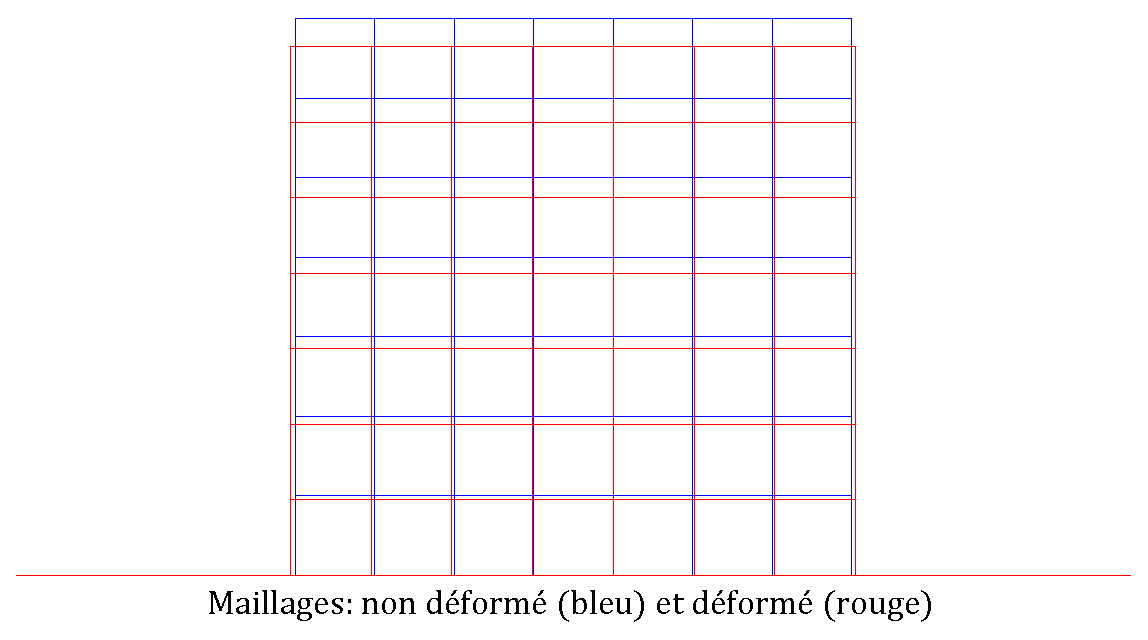
\includegraphics[height=40mm]{Contact1-def.eps}} \hfill
%  \subfloat[déplacement~$u_y$]{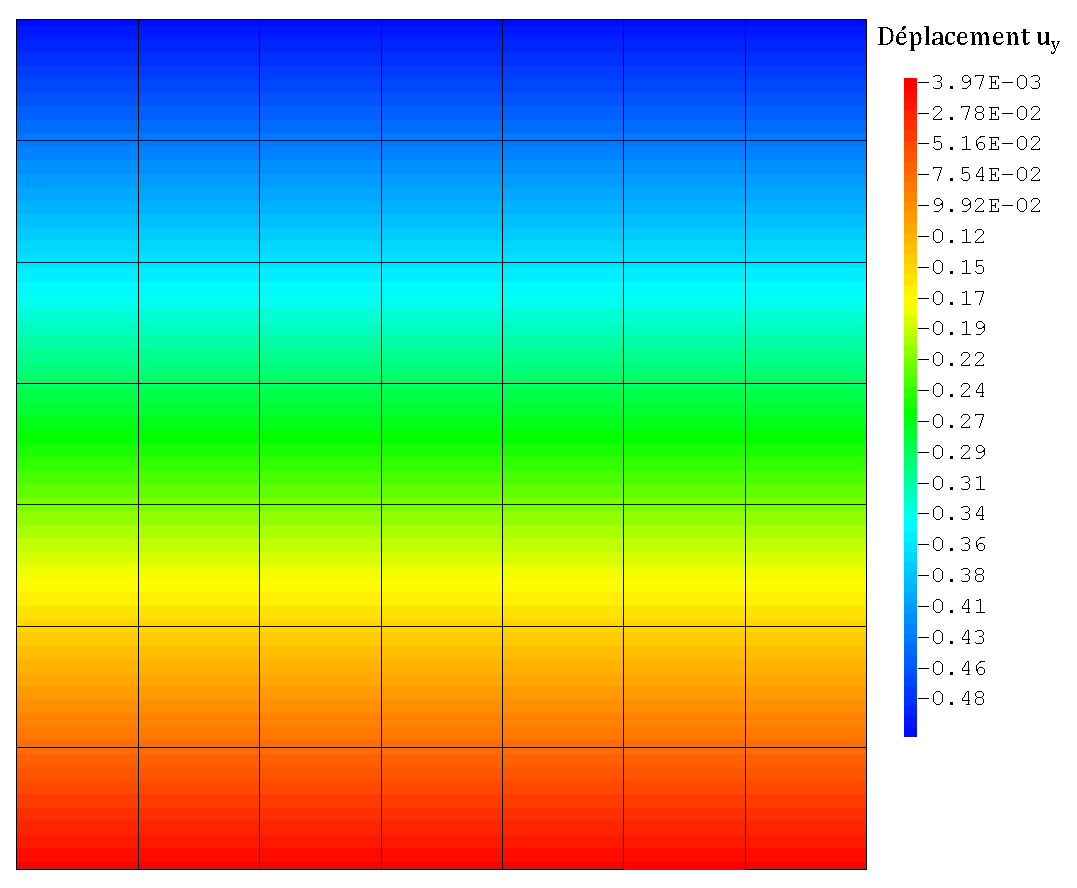
\includegraphics[height=40mm]{Contact1-uy.eps}}\hfill 
  \subfloat[forces de réactions]{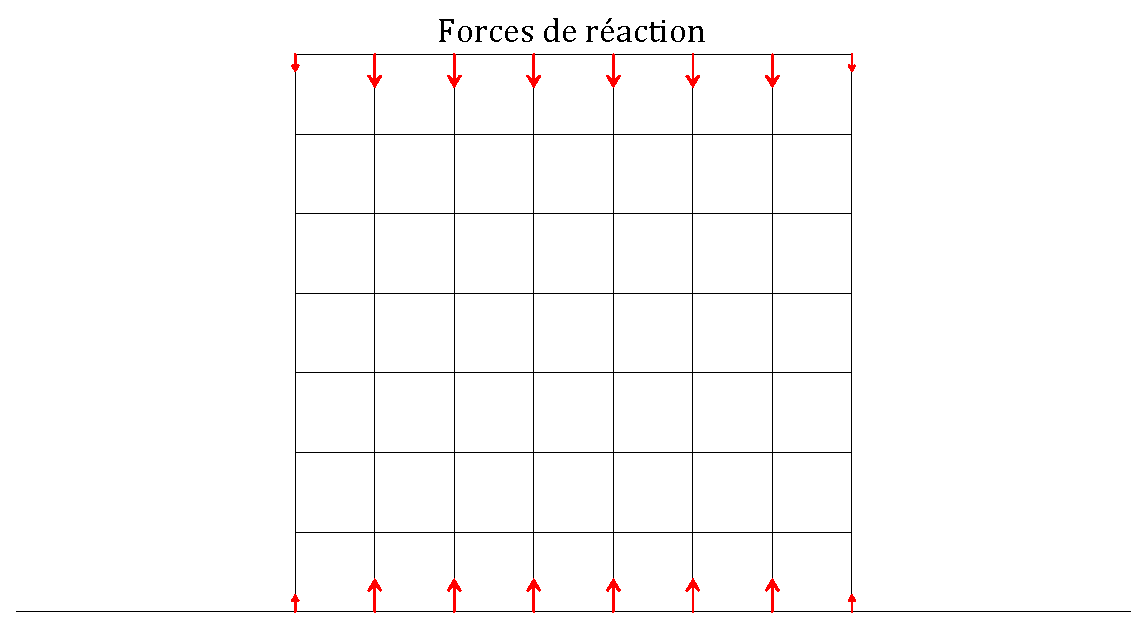
\includegraphics[height=40mm]{Contact1-reac.eps}}
  \caption{\label{Fig-Cont1} Premiers résultats sur le contact}
\end{figure}






\medskip
\subsection{Contact entre deux solides}

On peut faire une remarque sur le calcul précédent: que se passe-t-il si la surface sur laquelle on s'appuie n'est plus infiniment rigide ?

\medskip
On pourrait modéliser la partie inférieure et lui appliquer les forces de réactions qui ont été calculées précédemment.

Nous n'allons évidemment pas procéder ainsi et laisser \castem tout calculer pour nous...

\color{gris}\scriptsize
\begin{multicols}{2}
\begin{Verbatim}[numbers=left,numbersep=3pt]
OPTION ECHO 0 ;
OPTION DIME 2 ELEM QUA4 MODE PLAN CONT;
*
* Donnees
long1=10.;
nlong1=7;
uy0=-0.5;
haut1=long1;
nhaut1=nlong1;
jeu1=1.0;
*
* pave sur lequel le carre viendra buter:
k1 = (-1.*long1) 0.;
k2 = long1 0.;
l1 = DROI (2*nlong1-1) k2 k1;
s2 = l1 TRAN nhaut1 (0. (-1.0*haut1));
*
* carre
k3 = (-0.5*long1) jeu1;
k4 = (0.5*long1) jeu1;
l2 = DROI nlong1 k3 k4;
s1 = l2 TRAN nhaut1 (0. haut1);
trac (s1 et s2);
*
* Modele
ModM1 = MODEL s1 MECANIQUE ELASTIQUE;
MatM1 = MATER ModM1 'YOUN' 1.E3 'NU' 0.3 ;
ModM2 = MODEL s2 MECANIQUE ELASTIQUE;
MatM2 = MATER ModM2 'YOUN' 5.E3 'NU' 0.3 ;
*
* CL (Rigidites)
* 1) il faut une condition selon UX
k5 = s1 POIN PROC (0. jeu1);
CLk5 = BLOQ k5 UX;
* 2) ligne sur laquelle on impose le deplacement
l3 = s1 'COTE' 3;
CLl3 = BLOQ l3 UY ;
DCLl3  = DEPI CLl3 UY0;
* 3) encastrement sous la partie basse
l4 = s2 'COTE' 3;
CLl4 = BLOQ L4 DEPL;
* Totalite des conditions aux limites
CL0 = CLk5 ET CLl3 ET CLl4;
*
* RESOLUTION
Depl1 Rigid1 = IMPO l2 l1;
MR1=RIGID ModM1 MatM1;
MR2=RIGID ModM2 MatM2;
dep1 = RESO (MR1 ET MR2 ET CL0 ET Rigid1) DCLl3;
*
* Post-Traitement
*
* deformee:
defo0 = DEFO (s1 ET s2) dep1 0. 'BLEU' ;
defo1 = DEFO (s1 ET s2) dep1 1. 'ROUG' ;
TITR 'Maillages non deforme (bleu) et deforme (rouge)' ;
TRAC (defo0 ET defo1) ;
*
TITR 'Champ de deplacements.' ;
DeplY1 = EXCO Dep1 UY;
TRAC DeplY1 (s1 et s2);
*
* Comparaison des champs de contraintes:
Sig1 = SIGM (ModM1 ET ModM2) (MatM1 ET MatM2) Dep1;
TITR 'Champ de contraintes.' ;
TRAC sig1 (ModM1 ET ModM2);
*
fin;
\end{Verbatim}
\end{multicols}
\color{black}\normalsize

\medskip
Cette fois-ci, nous avons mis~$jeu_1$ a une valeur non nulle pour bien comprendre comment se fait la résolution de ce système numérique.

On obtient les résultats illustrés à la \fig{Fig-Cont21} pour la déformée et les forces de réactions et à la \fig{Fig-Cont22} pour les déplacements et contraintes.

\begin{figure}[ht]
  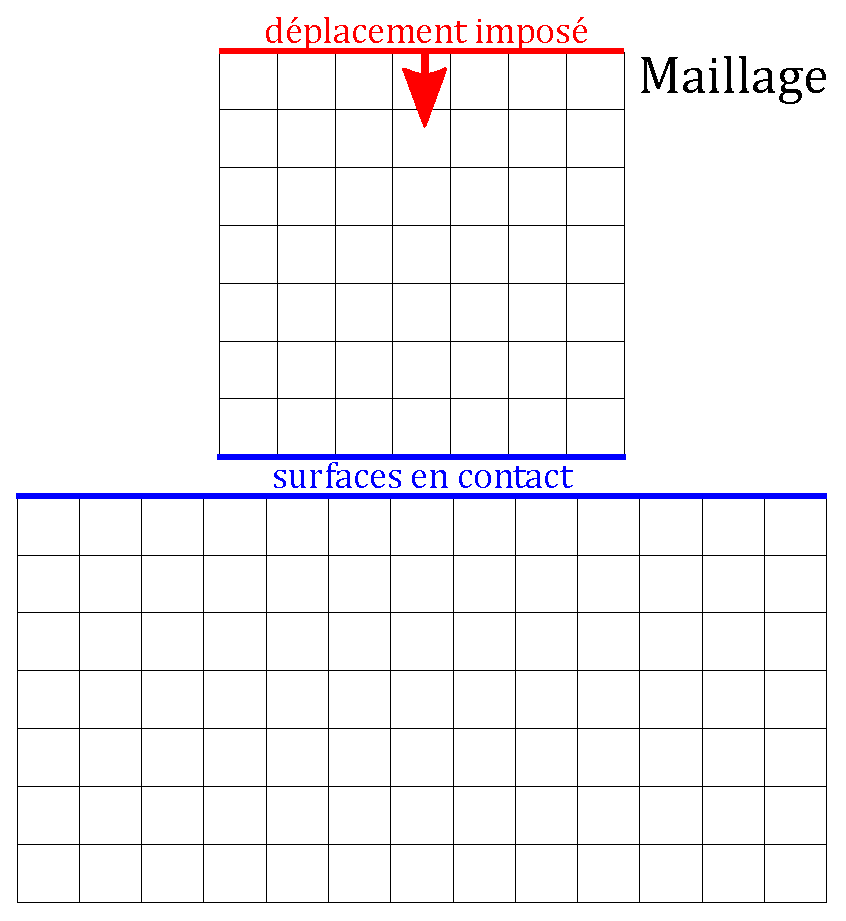
\includegraphics[height=40mm]{Contact2-pb.eps} \hfill 
  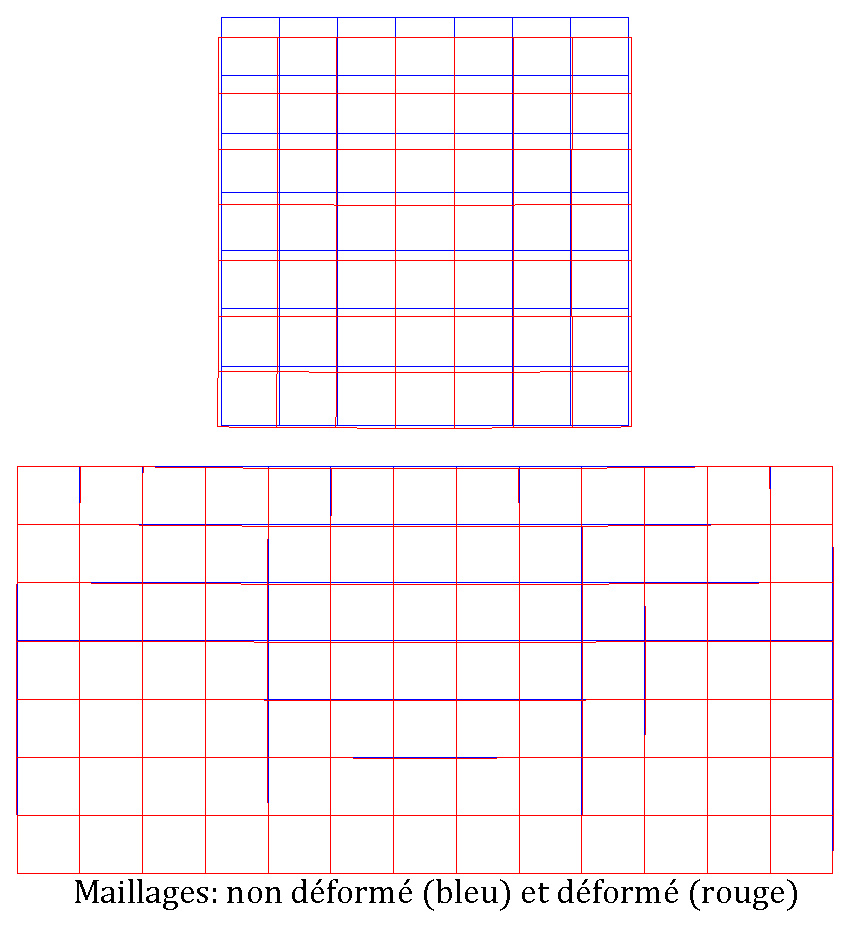
\includegraphics[height=40mm]{Contact2-def.eps}\hfill 
  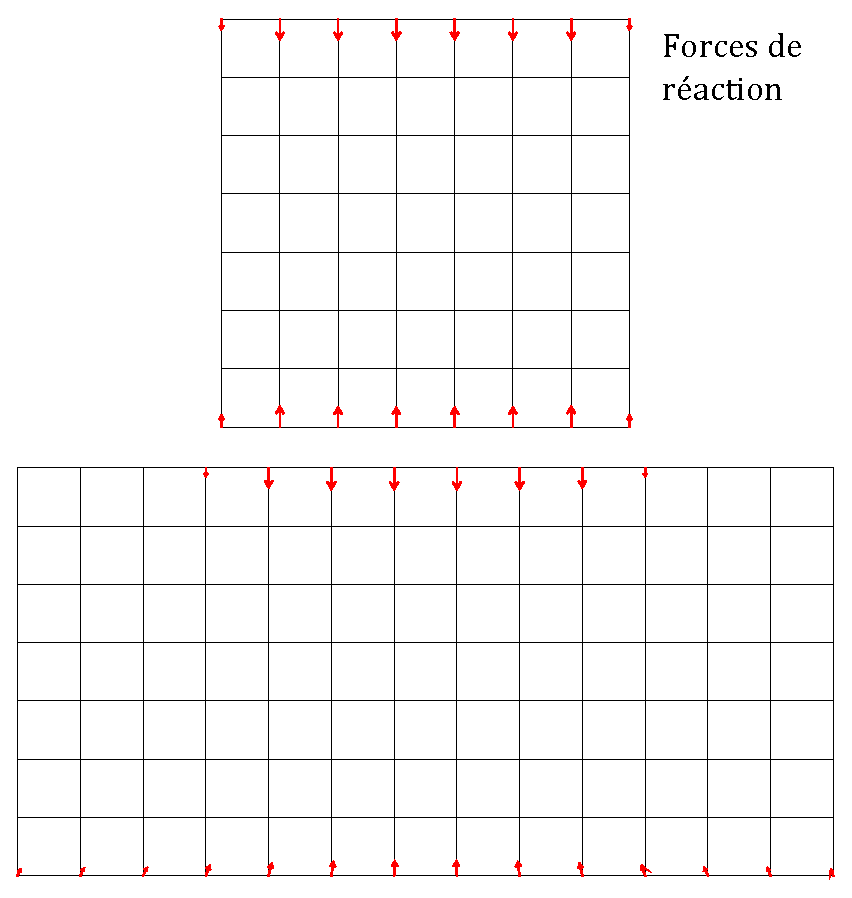
\includegraphics[height=40mm]{Contact2-reac.eps}
  \caption{\label{Fig-Cont21} a) maillage, b) déformée c) forces de réaction}
\end{figure}

\begin{figure}[ht]
  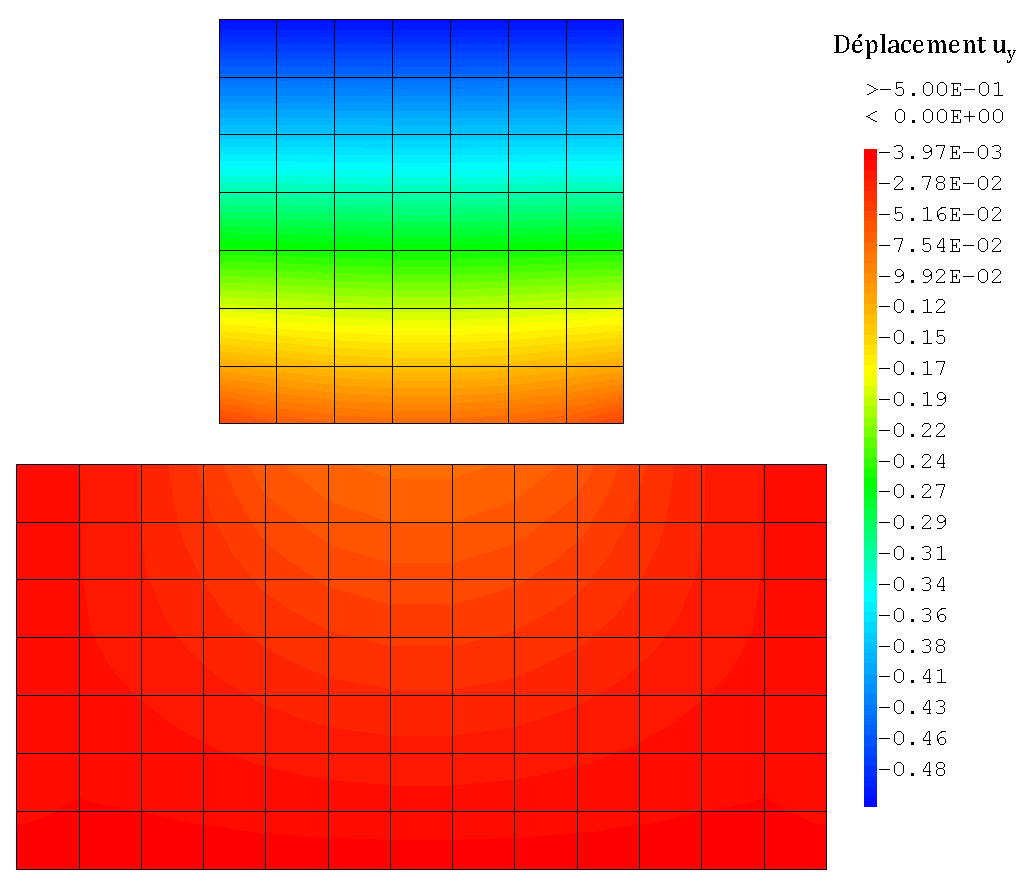
\includegraphics[height=40mm]{Contact2-uy.eps} \hfill 
  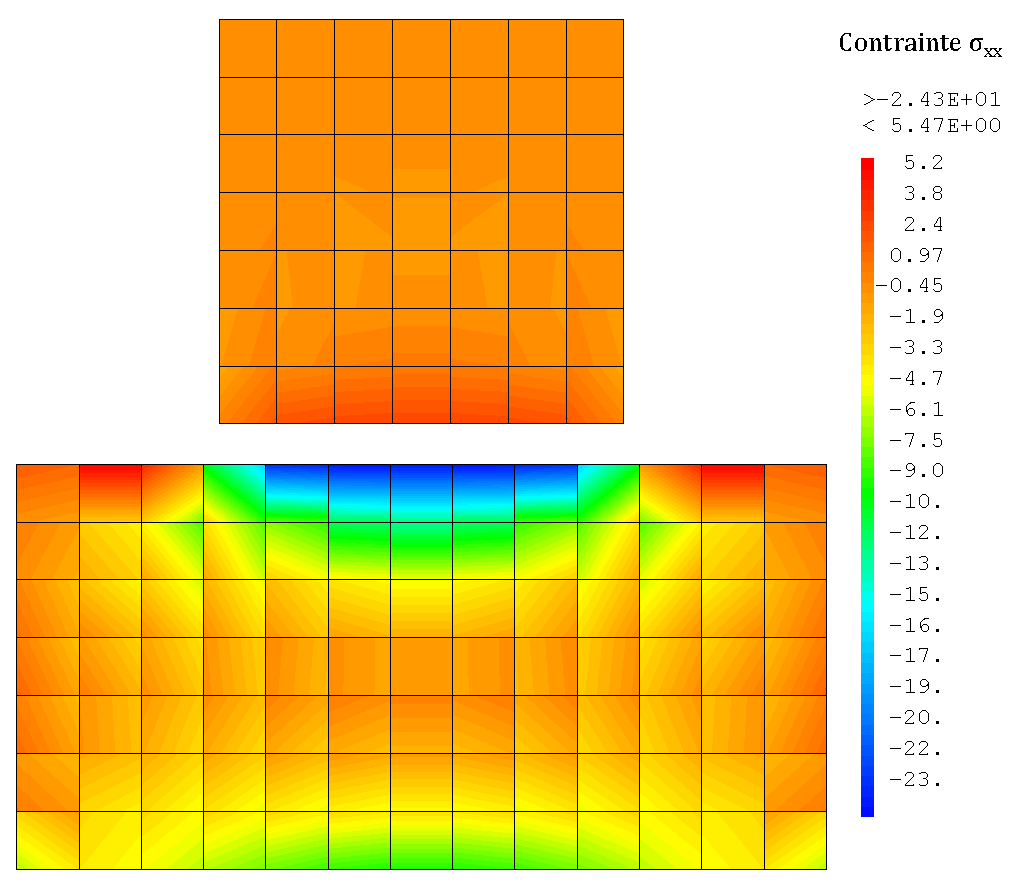
\includegraphics[height=40mm]{Contact2-sxx.eps}\hfill 
  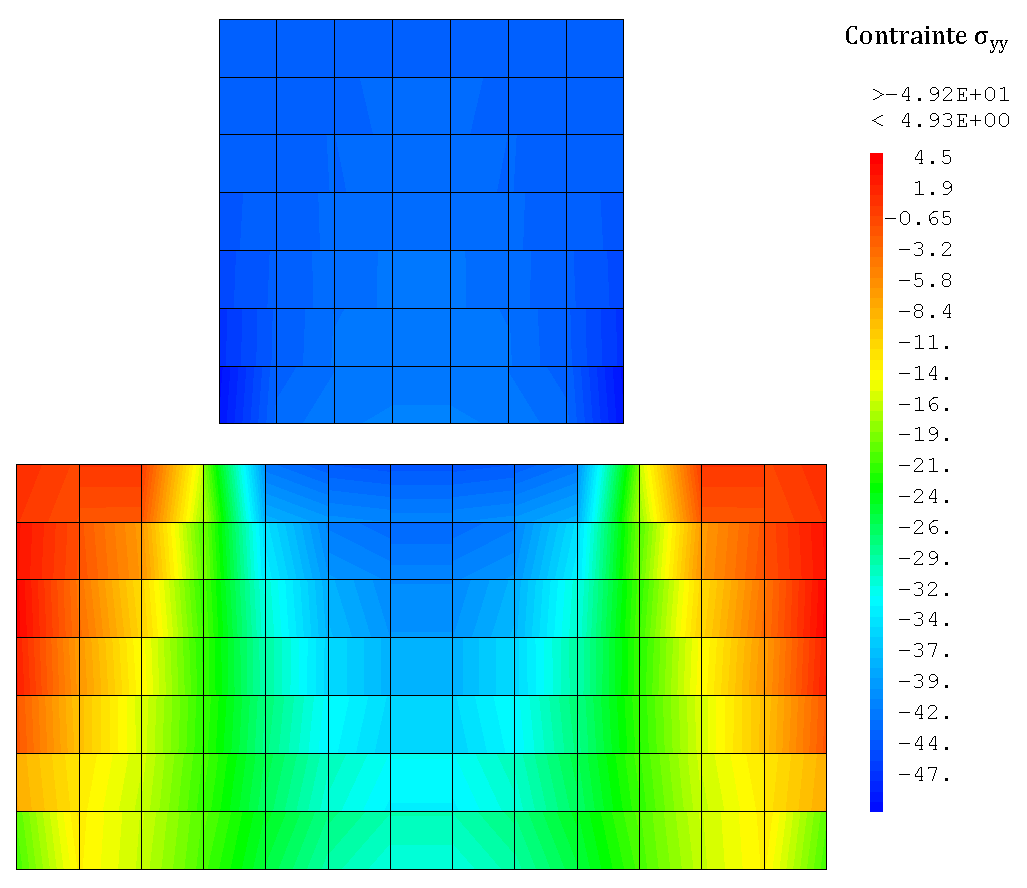
\includegraphics[height=40mm]{Contact2-syy.eps}
  \caption{\label{Fig-Cont22} a) déplacement~$u_y$ b)~$\sigma_{xx}$ et c)~$\sigma_{yy}$}
\end{figure}








\medskip
\subsection{Résolution pas à pas}

Les résolutions présentées ci-dessus étaient finalement de type classique, i.e. inversion d'un système comprenant les conditions aux limites et le chargement.

Cela fonctionnait particulièrement bien car nous étions en élasticité linéaire... mais que se passerait-il si le carré considéré avait un comportement non linéaire, en particulier s'il devait être le siège de déformations permanentes ?

On se doute aisément que le modèle rudimentaire ne fonctionnerait pas. C'est pourquoi nous allons le modifier afin d'introduire une résolution pas à pas, qui permet d'appliquer un chargement (ou un déplacement imposé) de manière progressive.

\medskip
Nous ne présentons pas ici de comportement non linéaire pour les matériaux, cela se fait en TD. Toutefois, nous présentons le même calcul que précédemment, mais codé pour une résolution pas à pas.

\medskip
Afin de définir le chargement dans le temps, nous commençons par construire la liste de réels~$Ltemp_1$ qui contient les pas de temps, à savoir~$0.0$ et~$1.0$ (2 pas de temps suffisent, puisque nous restons sur une analyse élastique linéaire dans cet exemple).

À partir de cette discrétisation du temps (vraiment sommaire pour le coup), nous définissons l'objet~$evo_1$ de type évolution pour chacun des pas de temps.~$evo_1$ est donc une fonction du temps, qui va nous servir à affecter le déplacement imposé:~$CharU_1$ est de type chargement, nécessaire pour la résolution par PASAPAS. Avec l'option DIMP, on signifie qu'il s'agit d'un déplacement imposé. Ainsi~$CharU_1$ contient l'évolution des déplacements imposés sur la condition DCLl3 au cours du temps.

\medskip
Les résultats sonr présentés à la \fig{Fig-Cont1}, après le listing.

\color{gris}\scriptsize
\begin{multicols}{2}
\begin{Verbatim}[numbers=left,numbersep=3pt]
OPTION ECHO 0 ;
OPTION DIME 2 ELEM QUA4 MODE PLAN CONT;
*
* Donnees
long1=10.;
nlong1=7;
uy0=-0.5;
haut1=long1;
nhaut1=nlong1;
jeu1=0.0;
*
* pave sur laquel le carre viendra buter:
k1 = (-1.*long1) 0.;
k2 = long1 0.;
l1 = DROI (2*nlong1-1) k2 k1;
s2 = l1 TRAN nhaut1 (0. (-1.0*haut1));
*
* carre
k3 = (-0.5*long1) jeu1;
k4 = (0.5*long1) jeu1;
l2 = DROI nlong1 k3 k4;
s1 = l2 TRAN nhaut1 (0. haut1);
trac (s1 et s2);
*
*
* Modele
ModM1 = MODEL s1 MECANIQUE ELASTIQUE;
MatM1 = MATER ModM1 'YOUN' 1.E3 'NU' 0.3 ;
ModM2 = MODEL s2 MECANIQUE ELASTIQUE;
MatM2 = MATER ModM2 'YOUN' 5.E3 'NU' 0.3 ;
*ModM1 = ModM1 ET ModM2;
*
* CL (Rigidites)
* 1) il faut une condition selon UX, on prend le point (0,0)
k5 = s1 POIN PROC (0. jeu1);
CLk5 = BLOQ k5 UX;
* 2) ligne sur laquelle on va imposer le deplacement
l3 = s1 'COTE' 3;
CLl3 = BLOQ l3 UY ;
DCLl3  = DEPI CLl3 UY0;
* 3) encastrement sous la partie basse
l4 = s2 'COTE' 3;
CLl4 = BLOQ L4 DEPL;
* 4) ligne de contact:
Depl1 Rigid1 = IMPO l2 l1;
*
* Totalite des conditions aux limites
CL0 = CLk5 ET CLl3 ET CLl4 ET Rigid1;
*
* Chargement
Ltemps1 = PROG 0. 1.;
evo1 = EVOL 'MANU' 'TEMPS' Ltemps1 (PROG 0. 1.) ;
CharU1 = CHAR DIMP DCLl3 evo1 ;
Char0 = CharU1 ;
*
* RESOLUTION
*
* Construction de la table PASAPAS:
TAB1            = TABL;
TAB1.'TEMPS_CALCULES'   = Ltemps1;
TAB1.'MODELE'       = (ModM1 ET ModM2);
TAB1.'CARACTERISTIQUES'  = (MatM1 ET MatM2);
TAB1.'BLOCAGES_MECANIQUES' = CL0;
TAB1.'CHARGEMENT'     = Char0;
*
* Resolution:
TAB2 = PASAPAS TAB1 ;
*
* Post-Traitement
*
dep1 = TAB2 . 'DEPLACEMENTS' . 1;
*
* deformee:
defo0 = DEFO (s1 ET s2) dep1 0. 'BLEU' ;
defo1 = DEFO (s1 ET s2) dep1 1. 'ROUG' ;
TITR 'Maillages non deforme (bleu) et deforme (rouge).' ;
TRAC (defo0 ET defo1) ;
*
TITR 'Champ de deplacements.' ;
DeplY1 = EXCO Dep1 UY;
TRAC DeplY1 (s1 et s2);
*
* Comparaison des champs de contraintes:
sig1 = TAB2 . 'CONTRAINTES' . 1 ;
TITR 'Champ de contraintes.' ;
TRAC sig1 (ModM1 ET ModM2);
*
* Visualisations des reactions:
reac1 = TAB2 . 'REACTIONS' . 1 ;
vr1 = VECT reac1 0.8E-2 'FX' 'FY' 'ROUG' ;
TITR 'Forces de reaction.' ;
TRAC vr1 (s1 ET s2) ;
*
fin;
\end{Verbatim}
\end{multicols}
\color{black}\normalsize

On obtient les mêmes résultats que ceux déjà présentés (voir \fig{Fig-Cont21} et \fig{Fig-Cont22}).

\bigskip
Nous pouvons mentionner également que ce type de calcul permet de calculer la géométrie de pièces réalisées en thermocompression. Considérons un matelas de matière souple placé entre le plateau supérieur d'une presse et un outil comportant un logement, comme illustré à la \fig{Fig-Thermo}a. Une fois que le plateau de presse est descendu, on obtient la pièce en forme donnée à la \fig{Fig-Thermo}b.

\begin{figure}[ht]
  \center
  \ifVersionDuDocEstVincent
     \includegraphics[width=80mm]{Thermo0.eps} \hfill
%     \includegraphics[height=40mm]{Thermo1.eps} \hfill
     \includegraphics[width=90mm]{Thermo2.eps}
  \else
     \includegraphics[width=64mm]{Thermo0.eps} \hfill
     \includegraphics[width=72mm]{Thermo2.eps}
  \fi
  \caption{\label{Fig-Thermo} Thermocompression: a) problème, b) forme de la pièce après production}
\end{figure}

\medskip
À partir des listings précédents, il est aisé d'obtenir les résultats de la \fig{Fig-Thermo}b... et nous vous invitons à le faire.

\medskip
Une fois ce premier calcul réalisé (et donc pleins de fierté et de confiance en nous), nous vous proposons d'utiliser un matelas de matière plus épais, \textcolorred{vraiment plus épais}. Le but est que lors du process, lorsque le plateau de la presse descend (situation réelle ou simulée), la matière vienne suffisamment remplir la cavité du moule pour qu'il y ait contact entre la pièce déformée et le fond de la cavité.

\bigskip
Nous allons alors constater que le contact n'est pris en compte que dans la partie supérieure du moule, mais pas sur les côtés de la cavité, ni au fond de celle-ci...

En TP, nous travaillerons à comprendre pourquoi (qu'est-ce que le code de calcul a compris de ce que nous lui avons proposé comme modélisation ?) et à réaliser un modèle correspondant à ce que nous souhaitions.
% contact Cast3M
\fi

